% Options for packages loaded elsewhere
\PassOptionsToPackage{unicode}{hyperref}
\PassOptionsToPackage{hyphens}{url}
\PassOptionsToPackage{dvipsnames,svgnames,x11names}{xcolor}
%
\documentclass[
  letterpaper,
  DIV=11,
  numbers=noendperiod]{scrreprt}

\usepackage{amsmath,amssymb}
\usepackage{iftex}
\ifPDFTeX
  \usepackage[T1]{fontenc}
  \usepackage[utf8]{inputenc}
  \usepackage{textcomp} % provide euro and other symbols
\else % if luatex or xetex
  \usepackage{unicode-math}
  \defaultfontfeatures{Scale=MatchLowercase}
  \defaultfontfeatures[\rmfamily]{Ligatures=TeX,Scale=1}
\fi
\usepackage{lmodern}
\ifPDFTeX\else  
    % xetex/luatex font selection
\fi
% Use upquote if available, for straight quotes in verbatim environments
\IfFileExists{upquote.sty}{\usepackage{upquote}}{}
\IfFileExists{microtype.sty}{% use microtype if available
  \usepackage[]{microtype}
  \UseMicrotypeSet[protrusion]{basicmath} % disable protrusion for tt fonts
}{}
\makeatletter
\@ifundefined{KOMAClassName}{% if non-KOMA class
  \IfFileExists{parskip.sty}{%
    \usepackage{parskip}
  }{% else
    \setlength{\parindent}{0pt}
    \setlength{\parskip}{6pt plus 2pt minus 1pt}}
}{% if KOMA class
  \KOMAoptions{parskip=half}}
\makeatother
\usepackage{xcolor}
\setlength{\emergencystretch}{3em} % prevent overfull lines
\setcounter{secnumdepth}{5}
% Make \paragraph and \subparagraph free-standing
\ifx\paragraph\undefined\else
  \let\oldparagraph\paragraph
  \renewcommand{\paragraph}[1]{\oldparagraph{#1}\mbox{}}
\fi
\ifx\subparagraph\undefined\else
  \let\oldsubparagraph\subparagraph
  \renewcommand{\subparagraph}[1]{\oldsubparagraph{#1}\mbox{}}
\fi

\usepackage{color}
\usepackage{fancyvrb}
\newcommand{\VerbBar}{|}
\newcommand{\VERB}{\Verb[commandchars=\\\{\}]}
\DefineVerbatimEnvironment{Highlighting}{Verbatim}{commandchars=\\\{\}}
% Add ',fontsize=\small' for more characters per line
\usepackage{framed}
\definecolor{shadecolor}{RGB}{241,243,245}
\newenvironment{Shaded}{\begin{snugshade}}{\end{snugshade}}
\newcommand{\AlertTok}[1]{\textcolor[rgb]{0.68,0.00,0.00}{#1}}
\newcommand{\AnnotationTok}[1]{\textcolor[rgb]{0.37,0.37,0.37}{#1}}
\newcommand{\AttributeTok}[1]{\textcolor[rgb]{0.40,0.45,0.13}{#1}}
\newcommand{\BaseNTok}[1]{\textcolor[rgb]{0.68,0.00,0.00}{#1}}
\newcommand{\BuiltInTok}[1]{\textcolor[rgb]{0.00,0.23,0.31}{#1}}
\newcommand{\CharTok}[1]{\textcolor[rgb]{0.13,0.47,0.30}{#1}}
\newcommand{\CommentTok}[1]{\textcolor[rgb]{0.37,0.37,0.37}{#1}}
\newcommand{\CommentVarTok}[1]{\textcolor[rgb]{0.37,0.37,0.37}{\textit{#1}}}
\newcommand{\ConstantTok}[1]{\textcolor[rgb]{0.56,0.35,0.01}{#1}}
\newcommand{\ControlFlowTok}[1]{\textcolor[rgb]{0.00,0.23,0.31}{#1}}
\newcommand{\DataTypeTok}[1]{\textcolor[rgb]{0.68,0.00,0.00}{#1}}
\newcommand{\DecValTok}[1]{\textcolor[rgb]{0.68,0.00,0.00}{#1}}
\newcommand{\DocumentationTok}[1]{\textcolor[rgb]{0.37,0.37,0.37}{\textit{#1}}}
\newcommand{\ErrorTok}[1]{\textcolor[rgb]{0.68,0.00,0.00}{#1}}
\newcommand{\ExtensionTok}[1]{\textcolor[rgb]{0.00,0.23,0.31}{#1}}
\newcommand{\FloatTok}[1]{\textcolor[rgb]{0.68,0.00,0.00}{#1}}
\newcommand{\FunctionTok}[1]{\textcolor[rgb]{0.28,0.35,0.67}{#1}}
\newcommand{\ImportTok}[1]{\textcolor[rgb]{0.00,0.46,0.62}{#1}}
\newcommand{\InformationTok}[1]{\textcolor[rgb]{0.37,0.37,0.37}{#1}}
\newcommand{\KeywordTok}[1]{\textcolor[rgb]{0.00,0.23,0.31}{#1}}
\newcommand{\NormalTok}[1]{\textcolor[rgb]{0.00,0.23,0.31}{#1}}
\newcommand{\OperatorTok}[1]{\textcolor[rgb]{0.37,0.37,0.37}{#1}}
\newcommand{\OtherTok}[1]{\textcolor[rgb]{0.00,0.23,0.31}{#1}}
\newcommand{\PreprocessorTok}[1]{\textcolor[rgb]{0.68,0.00,0.00}{#1}}
\newcommand{\RegionMarkerTok}[1]{\textcolor[rgb]{0.00,0.23,0.31}{#1}}
\newcommand{\SpecialCharTok}[1]{\textcolor[rgb]{0.37,0.37,0.37}{#1}}
\newcommand{\SpecialStringTok}[1]{\textcolor[rgb]{0.13,0.47,0.30}{#1}}
\newcommand{\StringTok}[1]{\textcolor[rgb]{0.13,0.47,0.30}{#1}}
\newcommand{\VariableTok}[1]{\textcolor[rgb]{0.07,0.07,0.07}{#1}}
\newcommand{\VerbatimStringTok}[1]{\textcolor[rgb]{0.13,0.47,0.30}{#1}}
\newcommand{\WarningTok}[1]{\textcolor[rgb]{0.37,0.37,0.37}{\textit{#1}}}

\providecommand{\tightlist}{%
  \setlength{\itemsep}{0pt}\setlength{\parskip}{0pt}}\usepackage{longtable,booktabs,array}
\usepackage{calc} % for calculating minipage widths
% Correct order of tables after \paragraph or \subparagraph
\usepackage{etoolbox}
\makeatletter
\patchcmd\longtable{\par}{\if@noskipsec\mbox{}\fi\par}{}{}
\makeatother
% Allow footnotes in longtable head/foot
\IfFileExists{footnotehyper.sty}{\usepackage{footnotehyper}}{\usepackage{footnote}}
\makesavenoteenv{longtable}
\usepackage{graphicx}
\makeatletter
\def\maxwidth{\ifdim\Gin@nat@width>\linewidth\linewidth\else\Gin@nat@width\fi}
\def\maxheight{\ifdim\Gin@nat@height>\textheight\textheight\else\Gin@nat@height\fi}
\makeatother
% Scale images if necessary, so that they will not overflow the page
% margins by default, and it is still possible to overwrite the defaults
% using explicit options in \includegraphics[width, height, ...]{}
\setkeys{Gin}{width=\maxwidth,height=\maxheight,keepaspectratio}
% Set default figure placement to htbp
\makeatletter
\def\fps@figure{htbp}
\makeatother

\KOMAoption{captions}{tableheading}
\makeatletter
\@ifpackageloaded{tcolorbox}{}{\usepackage[skins,breakable]{tcolorbox}}
\@ifpackageloaded{fontawesome5}{}{\usepackage{fontawesome5}}
\definecolor{quarto-callout-color}{HTML}{909090}
\definecolor{quarto-callout-note-color}{HTML}{0758E5}
\definecolor{quarto-callout-important-color}{HTML}{CC1914}
\definecolor{quarto-callout-warning-color}{HTML}{EB9113}
\definecolor{quarto-callout-tip-color}{HTML}{00A047}
\definecolor{quarto-callout-caution-color}{HTML}{FC5300}
\definecolor{quarto-callout-color-frame}{HTML}{acacac}
\definecolor{quarto-callout-note-color-frame}{HTML}{4582ec}
\definecolor{quarto-callout-important-color-frame}{HTML}{d9534f}
\definecolor{quarto-callout-warning-color-frame}{HTML}{f0ad4e}
\definecolor{quarto-callout-tip-color-frame}{HTML}{02b875}
\definecolor{quarto-callout-caution-color-frame}{HTML}{fd7e14}
\makeatother
\makeatletter
\@ifpackageloaded{bookmark}{}{\usepackage{bookmark}}
\makeatother
\makeatletter
\@ifpackageloaded{caption}{}{\usepackage{caption}}
\AtBeginDocument{%
\ifdefined\contentsname
  \renewcommand*\contentsname{Índice}
\else
  \newcommand\contentsname{Índice}
\fi
\ifdefined\listfigurename
  \renewcommand*\listfigurename{Lista de Figuras}
\else
  \newcommand\listfigurename{Lista de Figuras}
\fi
\ifdefined\listtablename
  \renewcommand*\listtablename{Lista de Tabelas}
\else
  \newcommand\listtablename{Lista de Tabelas}
\fi
\ifdefined\figurename
  \renewcommand*\figurename{Figura}
\else
  \newcommand\figurename{Figura}
\fi
\ifdefined\tablename
  \renewcommand*\tablename{Tabela}
\else
  \newcommand\tablename{Tabela}
\fi
}
\@ifpackageloaded{float}{}{\usepackage{float}}
\floatstyle{ruled}
\@ifundefined{c@chapter}{\newfloat{codelisting}{h}{lop}}{\newfloat{codelisting}{h}{lop}[chapter]}
\floatname{codelisting}{Listagem}
\newcommand*\listoflistings{\listof{codelisting}{Lista de Listagens}}
\makeatother
\makeatletter
\makeatother
\makeatletter
\@ifpackageloaded{caption}{}{\usepackage{caption}}
\@ifpackageloaded{subcaption}{}{\usepackage{subcaption}}
\makeatother
\ifLuaTeX
\usepackage[bidi=basic]{babel}
\else
\usepackage[bidi=default]{babel}
\fi
\babelprovide[main,import]{portuguese}
% get rid of language-specific shorthands (see #6817):
\let\LanguageShortHands\languageshorthands
\def\languageshorthands#1{}
\ifLuaTeX
  \usepackage{selnolig}  % disable illegal ligatures
\fi
\usepackage{bookmark}

\IfFileExists{xurl.sty}{\usepackage{xurl}}{} % add URL line breaks if available
\urlstyle{same} % disable monospaced font for URLs
\hypersetup{
  pdftitle={R e RStudio para Iniciantes},
  pdfauthor={GPEQ/UFRJ},
  pdflang={pt},
  colorlinks=true,
  linkcolor={blue},
  filecolor={Maroon},
  citecolor={Blue},
  urlcolor={Blue},
  pdfcreator={LaTeX via pandoc}}

\title{R e RStudio para Iniciantes}
\usepackage{etoolbox}
\makeatletter
\providecommand{\subtitle}[1]{% add subtitle to \maketitle
  \apptocmd{\@title}{\par {\large #1 \par}}{}{}
}
\makeatother
\subtitle{Material de Apoio para Cursos Quantitativos do Instituto de
Economia da Universidade Federal do Rio de Janeiro (IE/UFRJ)}
\author{GPEQ/UFRJ}
\date{2024-04-11}

\begin{document}
\maketitle

\renewcommand*\contentsname{Índice}
{
\hypersetup{linkcolor=}
\setcounter{tocdepth}{2}
\tableofcontents
}
\bookmarksetup{startatroot}

\chapter*{Prefácio}\label{sec-preface}
\addcontentsline{toc}{chapter}{Prefácio}

\markboth{Prefácio}{Prefácio}

\section*{O que você vai aprender}\label{o-que-vocuxea-vai-aprender}
\addcontentsline{toc}{section}{O que você vai aprender}

\markright{O que você vai aprender}

Pretendemos que você domine o \emph{mínimo} necessário de programação em
R para executar as tarefas que podem ser requisitadas pelo seu
professor, independentemente do curso da área quantitativa em que
estiver. Em outras palavras, se te pedirem algo que deva ser elaborado
com auxílio de programação em R, você será capaz de fazê-lo após ler
este material\footnote{Esperamos que os empecilhos que apareçam não
  sejam por conta de alguma dificuldade no ato de programar em si, mas
  por dúvidas com relação à matéria propriamente dita. De qualquer
  forma, fique tranquilo: se você não entendeu alguma parte do material,
  estaremos \textbf{sempre} abertos a te ajudar!}.

Na prática, o quê significa \emph{dominar o mínimo necessário de
programação em R?} Inclui entender alguns \emph{conceitos} básicos --
para quê serve a programação em nosso contexto, o que é a linguagem de
programação R, o que é o RStudio, entre outros -- assim como a
\emph{sintaxe} da linguagem -- ou seja, o ato de escrever um código
interpretável propriamente dito.

\section*{\texorpdfstring{O que você \textbf{não} vai
aprender}{O que você não vai aprender}}\label{o-que-vocuxea-nuxe3o-vai-aprender}
\addcontentsline{toc}{section}{O que você \textbf{não} vai aprender}

\markright{O que você \textbf{não} vai aprender}

Não estamos em um curso de Ciência da Computação: você não irá aprender
terminologias difíceis e/ou como a programação, de modo geral, funciona
nos \emph{detalhes}. Em outras palavras, vamos nos concentrar apenas em
entender o necessário para construir e executar \emph{códigos} em R (não
se preocupe, ainda explicaremos o que é um \emph{código em R}) a partir
das tarefas que seu professor poderá pedir.

Além disso, o material não te dará proficiência em R. O que queremos
dizer com isso? Bom, queremos dizer que você não será uma pessoa que
dominará o R de forma \emph{avançada}. Novamente: aqui, te ensinaremos
apenas o necessário para que consiga concluir os cursos da área
quantitativa. Mas, se você realmente quiser alcançar níveis mais altos,
alguns livros podem te ajudar:

\begin{itemize}
\item
  \href{https://r4ds.hadley.nz/}{R for Data Science (2ª edição)}
\item
  \href{https://livro.curso-r.com/index.html}{Ciência de Dados em R}
\item
  \href{https://bookdown.org/hneth/ds4psy/}{Data Science for
  Psychologists}
\item
  \href{https://bookdown.org/rwnahhas/IntroToR/}{An Introduction to R
  for Research}
\end{itemize}

\section*{Preciso saber alguma coisa de forma
antecipada?}\label{preciso-saber-alguma-coisa-de-forma-antecipada}
\addcontentsline{toc}{section}{Preciso saber alguma coisa de forma
antecipada?}

\markright{Preciso saber alguma coisa de forma antecipada?}

\textbf{Não}. Você não precisa saber absolutamente \emph{nada} de
programação em R -- não precisa nem mesmo saber o que o termo
\emph{programação} significa. O intuito do material é justamente te
introduzir aos conceitos mais básicos!

\textbf{A única coisa que você precisará será de acesso à um computador
com internet}. Utilizar um computador é necessário pois é nele onde
ocorre o ato de programar; ter internet é importante porquê, ao longo
dos captíulos, precisaremos que você realize o \emph{download} de certos
arquivos -- seja para instalar o R e o RStudio ou para \emph{importar}
algum arquivo diretamente para este último (não se preocupe, ainda
explicaremos o que \emph{importação} de um arquivo significa).

\section*{Como o material está
organizado}\label{como-o-material-estuxe1-organizado}
\addcontentsline{toc}{section}{Como o material está organizado}

\markright{Como o material está organizado}

O material está organizado em sete capítulos: o primeiro, que te mostra
a motivação para programar, além de outros seis que buscam, em primeiro
lugar, te guiar na instalação do R e RStudio e, na sequência, ensinar
comandos e conceitos básicos que serão necessários ao longo dos cursos.
Com intuito de facilitar o aprendizado, cada capítulo foi repartido em
um certo número de seções (e subseções, quando necessário).

A lista de capítulos pode ser observada no menu à \emph{esquerda}. Por
sua vez, a lista de seções do capítulo em que você estiver pode ser
observada no menu à \emph{direita}. Perceba que, para ser direcionado a
um determinado capítulo/seção, basta clicar em seu nome.

\begin{center}
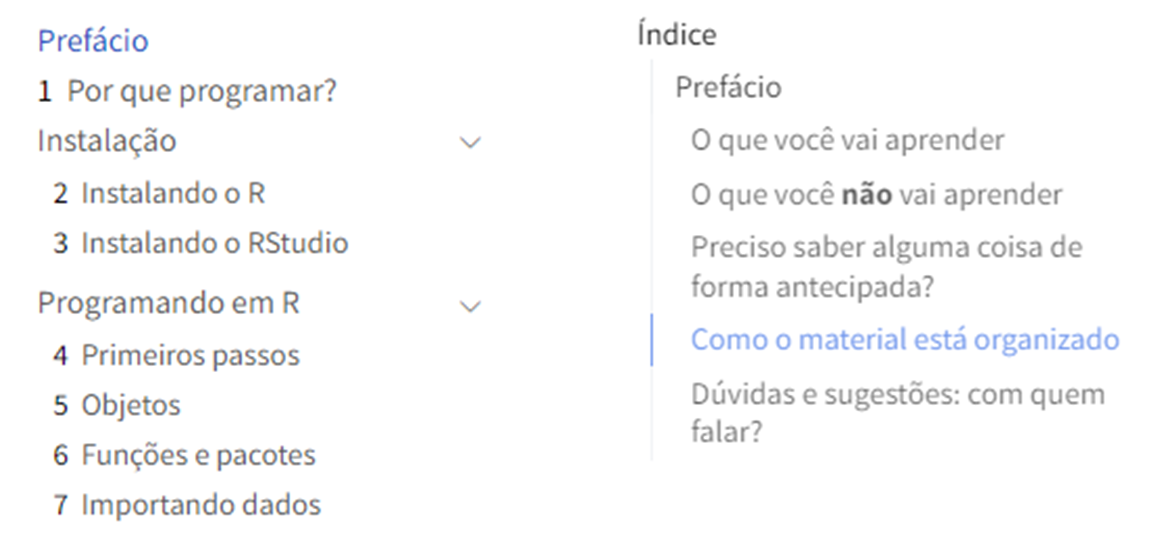
\includegraphics[width=5.63542in,height=\textheight]{images/clipboard-250739170.png}
\end{center}

\emph{``Caramba, queria tanto acessar uma parte específica do material
que não lembro muito bem onde está\ldots{} E agora?''} Sem problemas:
você pode pesquisar partes do texto ou palavras-chave no campo em branco
logo acima do Prefácio!

\begin{center}

\includegraphics[width=2.71875in,height=\textheight]{images/clipboard-2391069838.png}
\end{center}

\section*{Dúvidas e sugestões: com quem
falar?}\label{duxfavidas-e-sugestuxf5es-com-quem-falar}
\addcontentsline{toc}{section}{Dúvidas e sugestões: com quem falar?}

\markright{Dúvidas e sugestões: com quem falar?}

\emph{``Ué, no meu computador não aparece isso!''\\
``Caramba, achei aquele trechinho ali meio confuso\ldots{} podia
melhorar\ldots{}''\\
``Nossa, que material show!''}

Surgiu alguma dúvida ou então quer dar alguma sugestão de melhoria?
Estamos totalmente abertos à qualquer tipo de crítica! Envie uma
mensagem para \url{pedro.hemsley@ie.ufrj.br}.

\bookmarksetup{startatroot}

\chapter{Por que programar?}\label{sec-intro}

De forma simplificada, é possível definir o ato de programar como a
passagem de determinados comandos para o computador, com a finalidade de
que ele execute determinada tarefa. Se você deseja algo que pode ser
feito de forma mais eficiente por uma máquina, provavelmente escreverá
um código que seja interpretável por esta, de modo que seu desejo se
concretize.

A capacidade de programar tornou-se uma habilidade essencial,
especialmente para aqueles que desejam explorar o mundo da estatística e
da matemática aplicados à determinada ciência social. Por exemplo, no
contexto de interseção entre economia e matemática -- principalmente na
elaboração e solução de modelos teóricos -- e entre economia e
estatística -- testando hipóteses e realizando previsões -- a
programação se coloca como uma ferramenta muito útil para economizar
tempo de cálculo e garantir que, caso necessário, o mesmo processo seja
concluído múltiplas vezes sem erros. Em outras palavras, a programação
aplicada à determinada ciência social, como a economia, traz duas
principais vantagens, exploradas melhoras a seguir.

\section{Redução no tempo de
cálculo}\label{reduuxe7uxe3o-no-tempo-de-cuxe1lculo}

A primeira vantagem é a redução no tempo de cálculo de certos
procedimentos que, se feitos de forma manual, levariam vários minutos,
horas ou até mesmo dias. Vamos deixar mais claro com um exemplo.

No ensino fundamental, você aprendeu a resolver um sistema de equações
simultâneas com 2 variáveis e 2 equações, muito provavelmente pelo
método de substituição. Não levava muito tempo, certo? Acontece que, na
cadeira de Álgebra Linear, você aprenderá como solucionar sistemas de
\(n\) equações e \(n\) variáveis. Normalmente, quanto maior \(n\), maior
será a dificuldade de encontrar a solução do sistema. Ainda que existam
\emph{algoritmos} que permitam encontrar a solução de forma mais rápida,
certo tempo será perdido se você os replicar de forma \emph{manual}.

Com auxílio da programação, no entanto, é possível implementar estes
mesmos algoritmos para obter o resultado de forma quase que
\emph{instantânea.} \emph{O tempo que você levaria fazendo o
procedimento manual praticamente se reduz a zero -- ou fica mínimo, em
relação ao incial.} Observe que você ainda deve focar em saber como o
algoritmo funciona, do contrário não será capaz de julgar se o que a
máquina fez é realmente aquilo que você desejava.

\section{Automação de processos}\label{automauxe7uxe3o-de-processos}

Na seção anterior, repare que estavamos discorrendo implicitamente sobre
cálculos de ocorrência única -- ou seja, realizamos o cálculo uma vez e
não teríamos mais interesse de fazê-lo novamente em um futuro próximo.
No entanto, outro benefício prático do ato de programar é a automação de
tarefas repetitivas. Com a programação, é possível escrever e salvar
\emph{scripts} que automatizam tarefas tediosas de manipulação e análise
de dados, permitindo que os pesquisadores se concentrem em questões
analíticas de maior relevância.

Por exemplo, imagine que alguém te peça para calcular a média de certos
valores que mudam de dia para dia. Você pode facilmente elaborar um
\emph{scipt} que, a partir de determinados números (sem especificar
quais são), calcule sua média. Uma vez escrito e salvo, você pode passar
a executá-lo sempre que quiser -- no exemplo, todos os dias.

\section{Vamos programar!}\label{vamos-programar}

Em suma, aprender a programar oferece uma série de vantagens tangíveis
para quem trabalha com estatística e matemática. Ela tornar o trabalho
mais eficiente e produtivo, permitindo que os profissionais explorem
dados de maneiras antes inimagináveis e desenvolvam soluções
personalizadas para os desafios enfrentados em suas áreas de atuação.

No restante do material, aprenderemos a programar utilizando a
\emph{linguagem de programação R.} Em outras palavras, aprenderemos sua
\emph{sintaxe}, isto é, a forma de escrever comandos corretamente para
que a máquina seja capaz de interpretar e executar o que queremos como
resultado.

\part{Instalação}

Nessa parte, você irá aprender como baixar e instalar o R e o RStudio,
além da composição de \emph{layout} de ambos. Construímos cada seção de
instalação como um guia do tipo \emph{passo a passo}, de maneira que
você precisa apenas seguí-los de forma direta. Neste capítulo, é
importante que você já comece a explorar um pouco a interface dos
ambientes de programação que te mostraremos.

\chapter{Instalando o R}\label{instalando-o-r}

Nesse capítulo, iremos aprender como baixar e instalar o R para
Windows\footnote{Você pode realizar procedimento equivalente para
  sistemas operacionais Linux, apenas alterando a opção de
  \emph{download} quando necessário -- isto é, selecionando as opções em
  que esteja escrito `Linux', ao invés de `Windows'.}! Optamos por
dividir o passo a passo em 7 etapas -- mas fique tranquilo, não são
passos grandes, apenas fizemos dessa forma para que o conteúdo fique bem
\emph{mastigado}, fácil de entender.

\begin{tcolorbox}[enhanced jigsaw, colback=white, colframe=quarto-callout-tip-color-frame, colbacktitle=quarto-callout-tip-color!10!white, bottomrule=.15mm, opacityback=0, breakable, opacitybacktitle=0.6, left=2mm, titlerule=0mm, toptitle=1mm, bottomtitle=1mm, arc=.35mm, title=\textcolor{quarto-callout-tip-color}{\faLightbulb}\hspace{0.5em}{Alguns conceitos iniciais (Opcional)}, rightrule=.15mm, toprule=.15mm, leftrule=.75mm, coltitle=black]

Antes de começar, vamos entender alguns conceitos. A ideia aqui é te
ensinar o que significam algumas nomenclaturas e siglas que aparecem ao
longo do processo de instalação, em especial \emph{R Foundation} e
\emph{CRAN}. Essa parte é totalmente \emph{opcional} e você pode pular
direto para o passo a passo caso esteja sem tempo -- ou até mesmo
interesse.

\begin{itemize}
\item
  \textbf{R Foundation}: é uma empresa sem fins lucrativos, criada pelos
  principais desenvolvedores da linguagem. Quais são seus objetivos?
  Basicamente três: (i) administrar os direitos autorais da linguagem --
  e, por consequência, manter seu uso como livre; (ii) apoiar o
  desenvolvimento do R como um todo, isto é, fornecer informações e
  criar novos usos básicos, elaborar conferências, guias, entre outros;
  (iii) servir como ponto focal para todos os usuários da linguagem que
  desejem interagir com a comunidade de desenvolvedores. De forma
  resumida, a R Foundation é como se fosse a instituição provedora do
  básico da linguagem, que busca sempre atualizar e mantê-lo de pé. Se
  você instala o R e, logo em seguida, percebe que alguma de suas
  atribuições não está em perfeito funcionamento, provavelmente terá que
  comunicar à essas pessoas. Grosso modo, exerce um papel próximo ao da
  Microsoft com o Excel, por exemplo. Uma observação (importante): como
  o R é um software livre, qualquer pessoa pode desenvolver novas
  funções ou recursos a partir da linguagem. Por esse motivo, para
  recursos que estejam além da \emph{base do R}, você deve recorrer à
  quem os criou! Por exemplo, com relação ao RStudio (que conheceremos
  mais à frente), devemos nos reportar à empresa Posit, sua
  desenvolvedora. Na prática, raramente (para não dizer nunca) iremos
  reportar alguma coisa à R Foundation, mas sim aos desenvolvedores
  daquele pacote/extensão específico (fique tranquilo, explicaremos mais
  à frente o conceito de \emph{pacote} para a linguagem).
\item
  \textbf{CRAN} (Comprehensive R Archive Network): segundo o própio, é
  ``\emph{uma coleção de sites que carrega material idêntico,
  consistindo nas distribuições do R, extensões contriubídas,
  documentação e arquivos binários de R}''. \emph{`Meu Deus, o que isso
  significa?'} Simples: apenas uma coleção de endereços da internet em
  que podemos baixar a versão mais recente do R, assim como pacotes.
  Quem mantém o CRAN? Instituições voluntárias; em seus sites, a parte
  onde é possível baixar arquivos relacionados ao R é chamada de
  \emph{mirror}. E com quais recursos o CRAN se mantém? Com os da
  própria instituição participante (principalmente em termos de
  colaboradores) e, também, da R Foundation!
\end{itemize}

Essa história toda para dizer: \textbf{o arquivo básico que iremos
baixar para instalar o R será obtido através de algum \emph{mirror} do
CRAN, isto é, a parte do site de alguma instituição voluntária em
colaboração com a R Foundation.}

\end{tcolorbox}

\section{Sete passos}\label{sete-passos}

\begin{enumerate}
\def\labelenumi{\arabic{enumi}.}
\item
  O primeiro passo consiste em escolher um repositório (\emph{mirror)}
  para baixar o R. No endereço
  \url{https://cran.r-project.org/mirrors.html} encontramos todas as
  opções disponíveis, por país e em ordem alfabética. No seu computador,
  deverá aparecer a seguinte tela:

  \begin{center}
  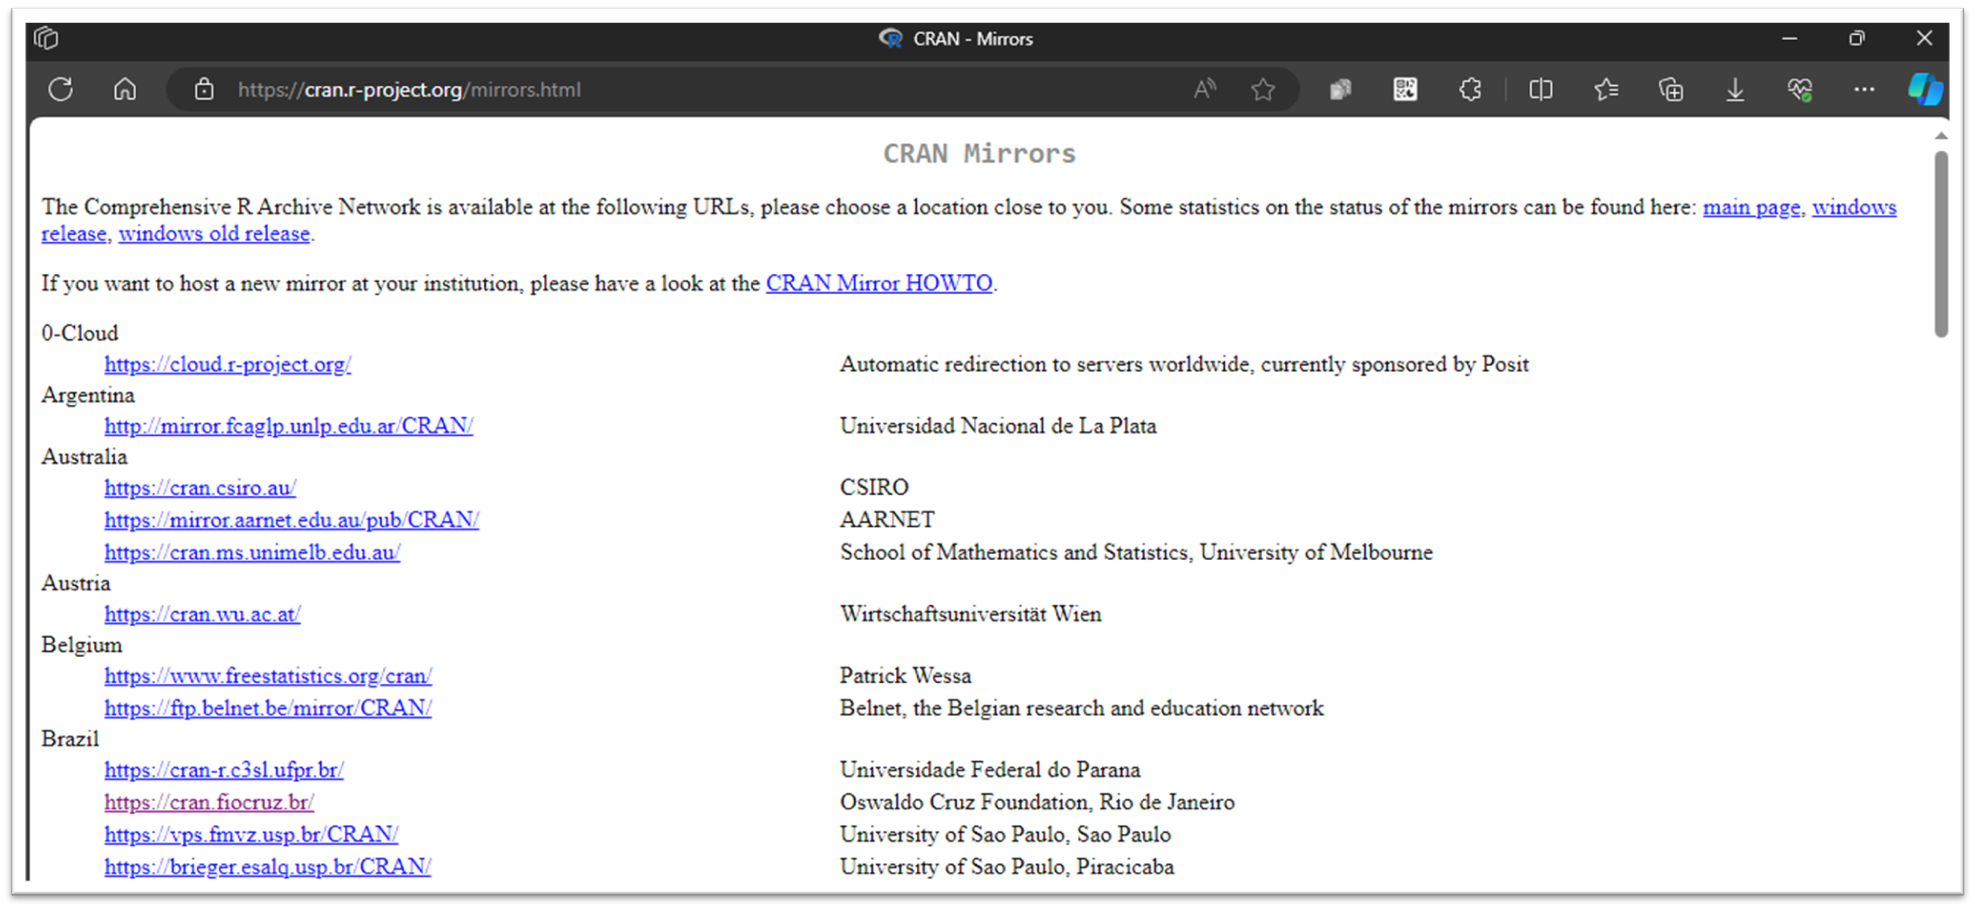
\includegraphics{images/clipboard-3074288328.png}
  \end{center}
\item
  Por questões de rapidez/latência, o ideal é escolher o repositório
  mais próximo de você. Considerando que todos estejam no Rio de
  Janeiro, vamos então utilizar o \emph{mirror} da Fiocruz.

  \begin{center}
  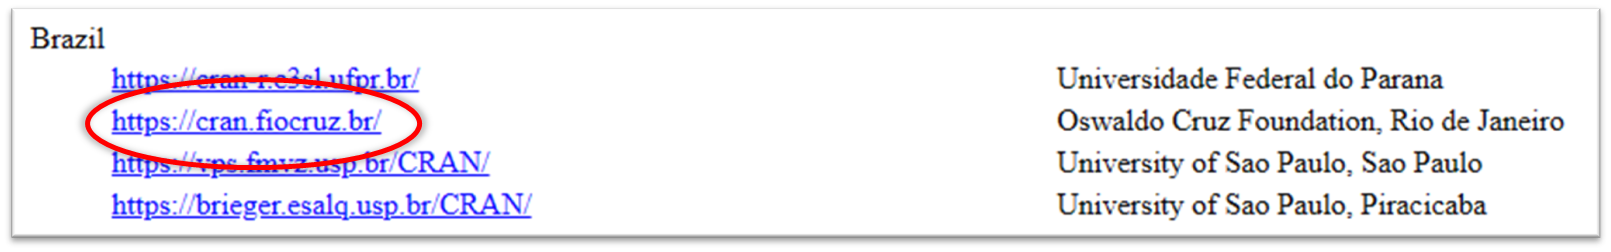
\includegraphics{images/clipboard-283220567.png}
  \end{center}
\item
  Como essa apostila foca na instalação para sistemas operacionais do
  tipo Windows, vamos clicar então em \emph{Download R for Windows}, na
  parte superior da página.

  \begin{center}
  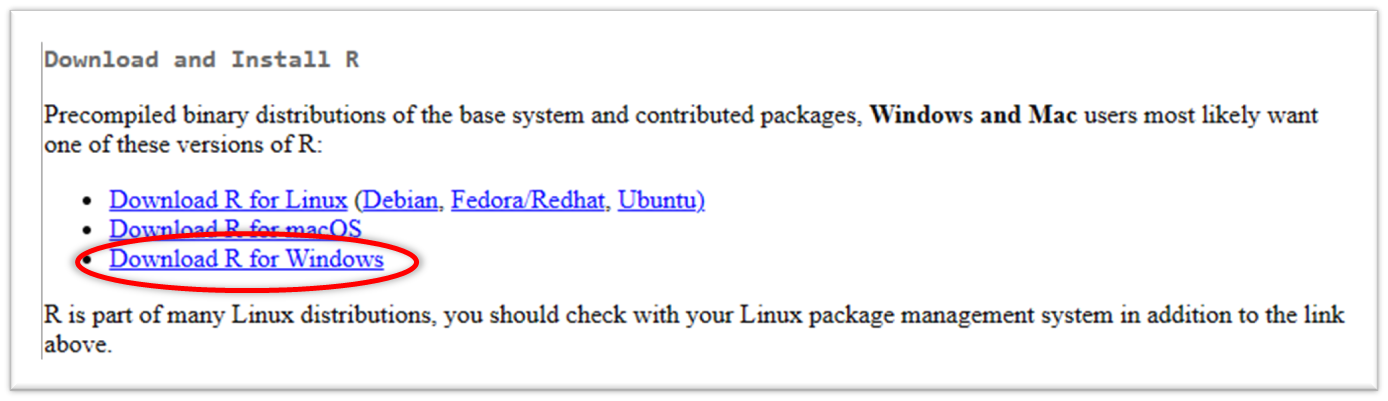
\includegraphics{images/clipboard-1477947543.png}
  \end{center}
\item
  Na página seguinte, clique em `base'. Grosso modo, como o nome já
  indica, iremos baixar os aquivos \emph{base} do R -- ou seja, o mínimo
  necessário que você precisará para poder executar algum código.

  \begin{center}
  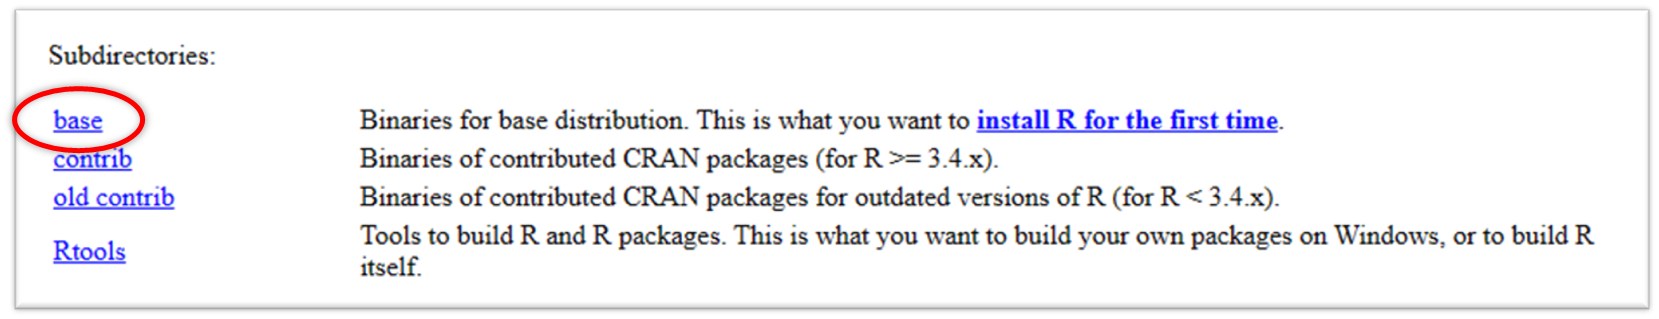
\includegraphics{images/clipboard-959933518.png}
  \end{center}
\item
  Na nova página, clique em `\emph{Download R x.x.x for Windows}', sendo
  `x.x.x' o número da versão que será baixada. No momento da elaboração
  deste tutorial, a versão mais recente do R é a 4.3.3.

  \begin{center}
  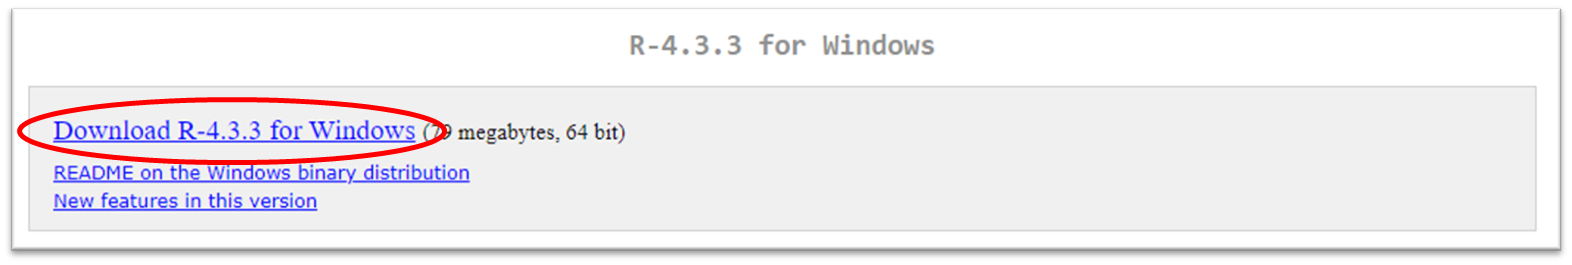
\includegraphics{images/clipboard-3581535596.png}
  \end{center}

  Se você tiver algum problema com o \emph{download}, tente escolher
  outro servidor no passo 2 -- por exemplo, um dos servidores da
  Universidade de São Paulo.
\end{enumerate}

\begin{tcolorbox}[enhanced jigsaw, colback=white, colframe=quarto-callout-note-color-frame, colbacktitle=quarto-callout-note-color!10!white, bottomrule=.15mm, opacityback=0, breakable, opacitybacktitle=0.6, left=2mm, titlerule=0mm, toptitle=1mm, bottomtitle=1mm, arc=.35mm, title=\textcolor{quarto-callout-note-color}{\faInfo}\hspace{0.5em}{Encontrando o caminho!}, rightrule=.15mm, toprule=.15mm, leftrule=.75mm, coltitle=black]

Abaixo, os passos 1-5 para realizar o \emph{donwload}.

\begin{center}
\includegraphics[width=3.96875in,height=\textheight]{images/instalacao_r.gif}
\end{center}

\end{tcolorbox}

\begin{enumerate}
\def\labelenumi{\arabic{enumi}.}
\setcounter{enumi}{5}
\item
  Você receberá um aviso, que varia conforme o navegador em uso, de que
  o arquivo está sendo baixado. Abaixo, um exemplo no Microsoft Edge:

  \begin{center}
  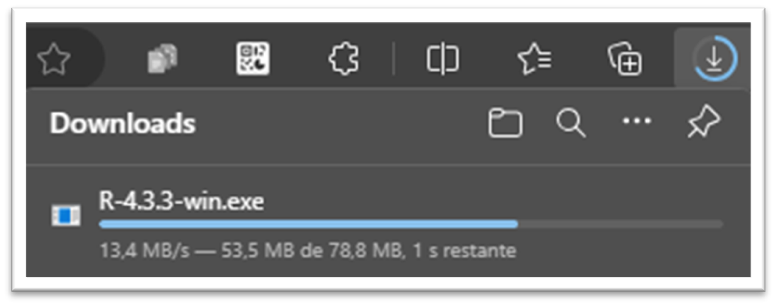
\includegraphics[width=3.96875in,height=\textheight]{images/clipboard-2313357345.png}
  \end{center}

  No Windows, o arquivo será armazenado na pasta `Downloads' do seu
  computador (ou na pasta que você previamente configurou como destino
  para os arquivos baixados).
\item
  Feito o download, clique duas vezes no arquivo baixado e siga as
  instruções para instalação. Na prática, basta clicar em `Avançar' até
  o fim.

  \begin{center}
  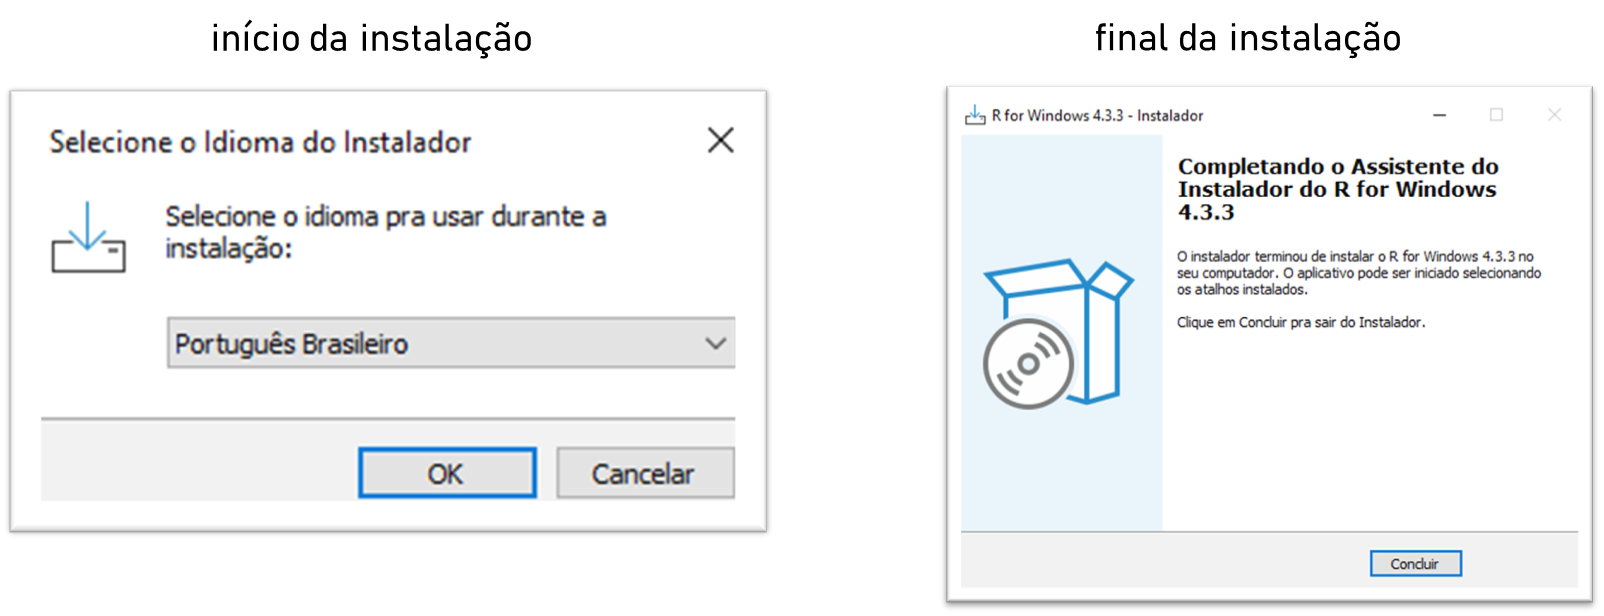
\includegraphics{images/clipboard-1694765597.png}
  \end{center}
\end{enumerate}

Após o final da instalação, você deverá ser capaz de encontrar e abrir
no seu computador o \textbf{R Graphical User Interface} ou, como
popularmente é conhecido, \textbf{RGui}. Ele estará na pasta em que você
destinou para instalação; no Windows, algo próximo de:

\texttt{C:\textbackslash{}ProgramData\textbackslash{}Microsoft\textbackslash{}Windows\textbackslash{}Start\ Menu\textbackslash{}Programs\textbackslash{}R}

\begin{center}
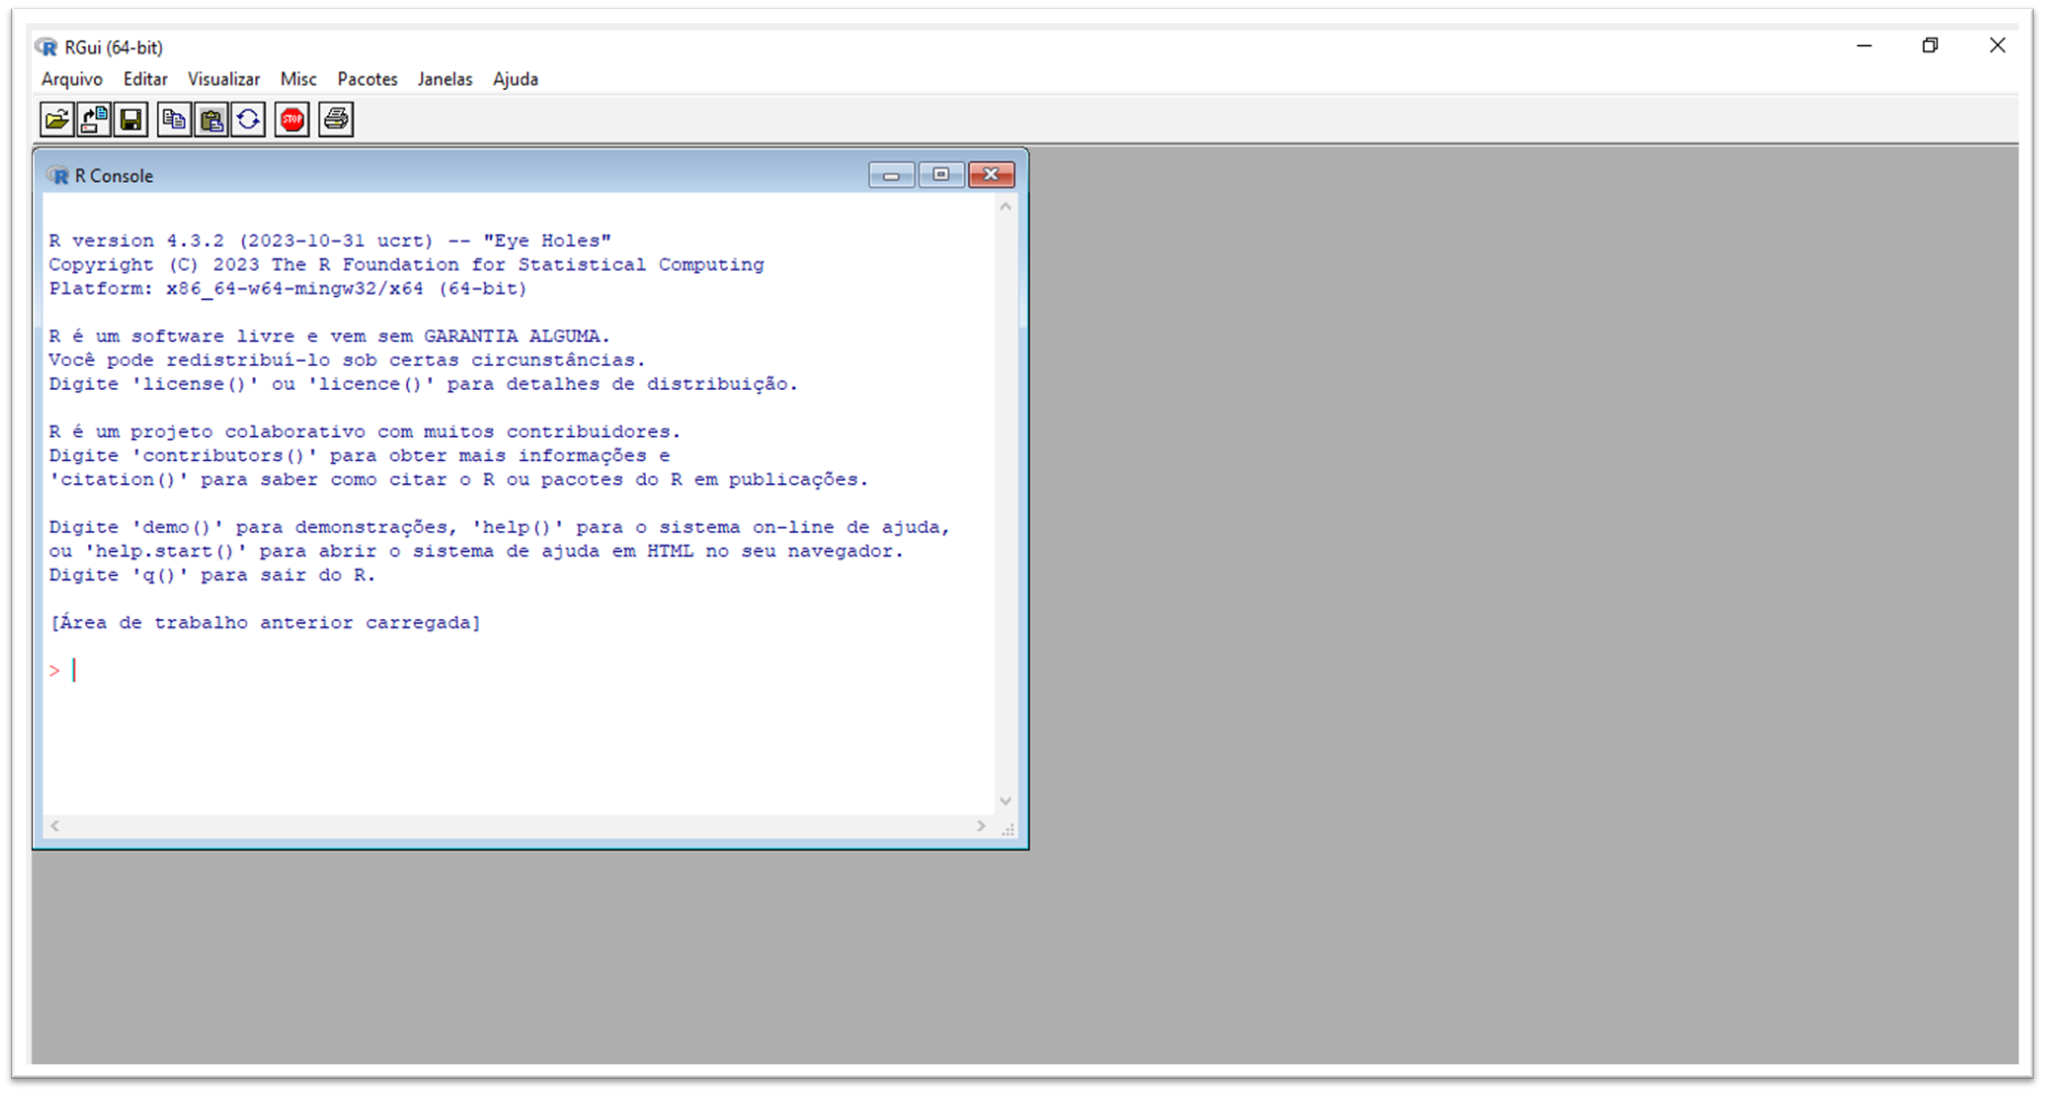
\includegraphics{images/clipboard-2094164095.png}
\end{center}

\section{Conhecendo o RGui}\label{conhecendo-o-rgui}

De forma geral, um GUI permite com que o usuário utilize a linguagem de
forma interativa através de botões e dispositivos visuais. Observe que,
na parte superior, temos oito botões principais, representados por
pequenas imagens.

\begin{center}
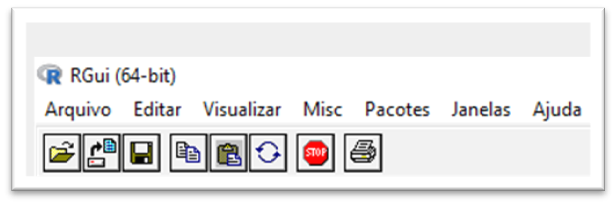
\includegraphics[width=3.125in,height=\textheight]{images/clipboard-3228534230.png}
\end{center}

Cada botão executa uma tarefa específica. Os três primeiros, da esquerda
para direita, são os mais relevantes:

\begin{itemize}
\item
  `Abrir script': permite com que você carregue, no Editor de Código, um
  arquivo que contém linhas de código (script). Arquivos desse tipo,
  cuja extensão é \texttt{.R}, serão os mais importantes da linguagem.
\item
  `Carregar área de trabalho': \emph{importa} objetos que foram salvos
  anteriormente em um arquivo do tipo \texttt{.RData}.
\item
  `Salvar área de trabalho': salva objetos criados em um arquivo do tipo
  \texttt{.RData}.
\end{itemize}

Os botões restantes, em ordem, executam as seguintes tarefas: `Copiar',
`Colar', `Copiar e colar', `Parar computação atual' e `Imprimir'. Nesse
momento, não se preocupe em saber o que significa \emph{importar} ou o
que é um arquivo do tipo \emph{.RData}.

Por outro lado, vamos procurar entender melhor o que são o
\textbf{Console} e o \textbf{Editor de Código}. O primeiro corresponde à
janela de nome \emph{R Console,} no canto esquerdo da sua tela. Este
último, por sua vez, não abre instantâneamente no momento em que você
acessa o RGui, mas podemos abrí-lo manualmente através de `Arquivo'
\textgreater{} `Novo script' -- ou, então, carregando um script já
existente através do botão `Abrir script', que vimos anteriormente.
Posicionando o Editor de Código ao lado do Console, teremos a seguinte
imagem:

\begin{center}
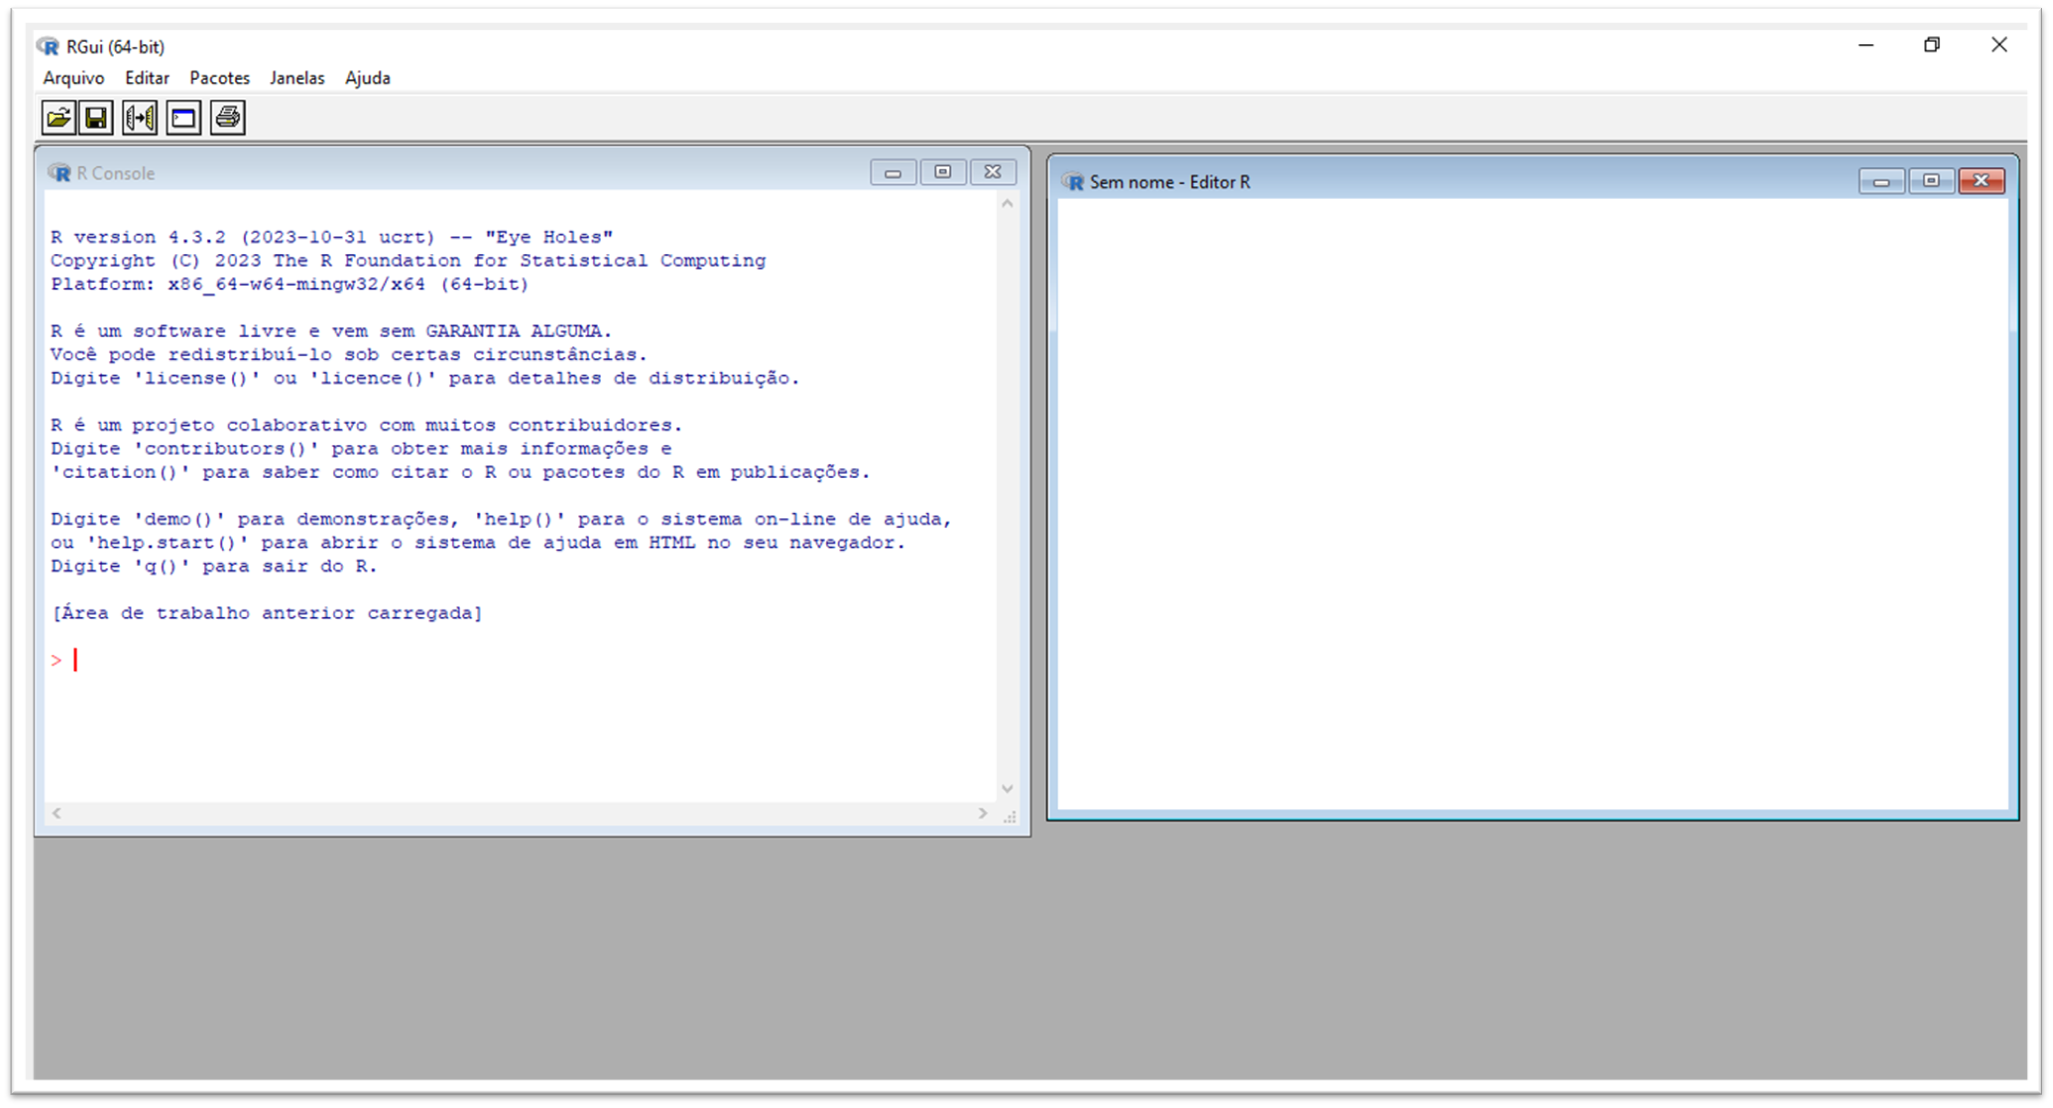
\includegraphics{images/clipboard-1401293353.png}
\end{center}

Por quê esses espaços terão relevância para nós?

\begin{itemize}
\item
  O Editor de Código é o local em que você escreve os comandos que
  deseja executar no R, além de comentários que busquem registrar o
  porquê de você ter escrito determinada parte do seu código. Na
  prática, um \emph{comentário} é uma linha que não será interpretada --
  e consequentemente executada -- como parte da linguagem. Para
  registrar um comentário, basta escrever o símbolo `\#' antes do que
  você deseja escrever naquela linha\footnote{Note que, se o seu
    comentário for longo demais, de tal forma que você queira quebrá-lo
    em duas ou mais linhas, será necessário novamente escrever `\#' na
    próxima linha}. Um ponto importante: o Editor permite com que
  salvemos o script que criamos em um arquivo do tipo \texttt{.R}.
  Lembre-se: esse é o principal tipo de arquivo da linguagem.
\item
  O Console, por sua vez, é o local em que a parte interpretável de
  código em R (ou seja, tudo exceto comentários) será
  \emph{efetivamente} executada e os respectivos resultados serão
  mostrados. É aqui que a mágica efetivamente ocorre! Você também pode
  executar partes do seu código diretamente no Console, porém os
  comandos não ficam salvos, são apenas temporários.
\end{itemize}

Simplificando: \textbf{o Editor é o espaço em que você realmente
escreverá os códigos em R}. Ele atua como rascunho do seu script,
permitindo com que você posteriormente salve o que foi escrito e,
consequentemente, volte a executar o mesmo código. Já \textbf{o Console
é o espaço em que o código é processado, retornando com o resultado dos
comandos que você escreveu}.

\textbf{Entretanto, não iremos utilizá-los através do RGui.} No capítulo
seguinte, instalaremos e conheceremos um pouco mais sobre outro
ambiente, bem mais completo, para se programar em R. \emph{``Meu Deus,
aprendi todos esses conceitos à toa?''}, você deve estar se perguntando.
Não! Muito do que aprendemos nessa seção voltará a aparecer no capítulo
seguinte.

\begin{tcolorbox}[enhanced jigsaw, colback=white, colframe=quarto-callout-tip-color-frame, colbacktitle=quarto-callout-tip-color!10!white, bottomrule=.15mm, opacityback=0, breakable, opacitybacktitle=0.6, left=2mm, titlerule=0mm, toptitle=1mm, bottomtitle=1mm, arc=.35mm, title=\textcolor{quarto-callout-tip-color}{\faLightbulb}\hspace{0.5em}{Executando um simples código no RGui (Opcional)}, rightrule=.15mm, toprule=.15mm, leftrule=.75mm, coltitle=black]

Beleza, não tocaremos no RGui. Mas é interessante compreender que já é
possível executar -- ou \emph{rodar,} no jargão de programação -- algum
pedaço de código -- ou \emph{chunk} -- escrito em R. Para isso, basta
escrevê-lo após o símbolo de `maior que' (\textgreater) no Console.

Vamos entender com um rápido exemplo. No GIF abaixo, atribuimos à
variável de nome \texttt{x} o valor númerico \texttt{2}. Em seguida,
escrevemos o nome novamente para retornar seu valor. Fique tranquilo:
ainda iremos ver melhor o que significam termos como \emph{atribuir um
valor à determinada variável}. O objetivo deste \emph{box} foi apenas te
mostrar que já estamos aptos a programar em R!

\begin{center}
\includegraphics{images/rgui_exemplo.gif}
\end{center}

\end{tcolorbox}

\chapter{Instalando o RStudio}\label{instalando-o-rstudio}

\textbf{Acontece que o RGui não é tão prático de se usar}. Pensando
nisso, a empresa \href{https://posit.co/}{Posit} criou um Ambiente de
Desenvolvimento Integrado (\emph{Integrated Development Environment},
IDE) chamado \textbf{RStudio}. Em nosso contexto, tanto GUI quanto IDE
são ferramentas que permitem a utilização da linguagem. A diferença é
que a IDE tem atributos com a finalidade de facilitar o desenvolvimento
dos códigos. Grosso modo, toda IDE é uma GUI mas o inverso não é
verdadeiro (nem toda GUI é uma IDE).

Em resumo: \textbf{é muito mais fácil utilizar o R através do RStudio e,
por este motivo, vamos baixá-lo na sua versão gratuita} (que já é
suficiente para os cursos que serão ministrados no Instituto).

\section{Três passos}\label{truxeas-passos}

Para instalar o RStudio no Windows, novamente iremos seguir alguns
passos -- nesse caso, apenas 3:

\begin{enumerate}
\def\labelenumi{\arabic{enumi}.}
\item
  Acesse a página de downloads da RStudio:
  \url{https://posit.co/download/rstudio-desktop/\#download}. Se você
  tiver acesso de administrador, basta clicar em \emph{`Download RStudio
  Desktop for Windows'}.

  \begin{center}
  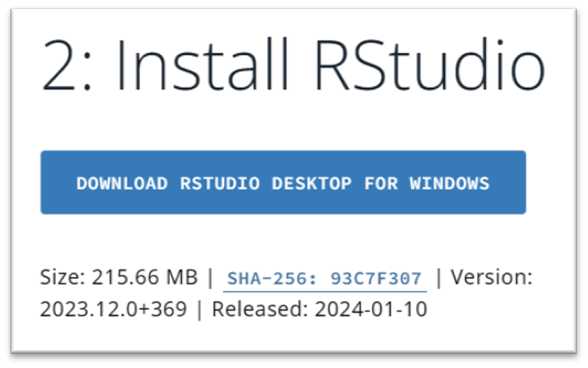
\includegraphics[width=3.32292in,height=\textheight]{images/clipboard-2426047081.png}
  \end{center}
\item
  De forma análoga ao \emph{download} do R, você receberá um aviso de
  que o arquivo está sendo baixado (na sua pasta de `Downloads' ou
  similar).

  \begin{center}
  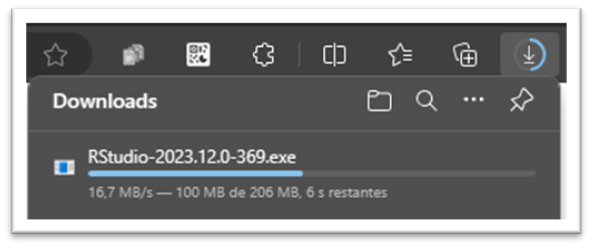
\includegraphics[width=3.85417in,height=\textheight]{images/clipboard-3795362132.png}
  \end{center}
\item
  Clique duas vezes no arquivo que você baixou e siga as instruções
  recomendadas de instalação, cuja tela inicial está na imagem abaixo.

  \begin{center}
  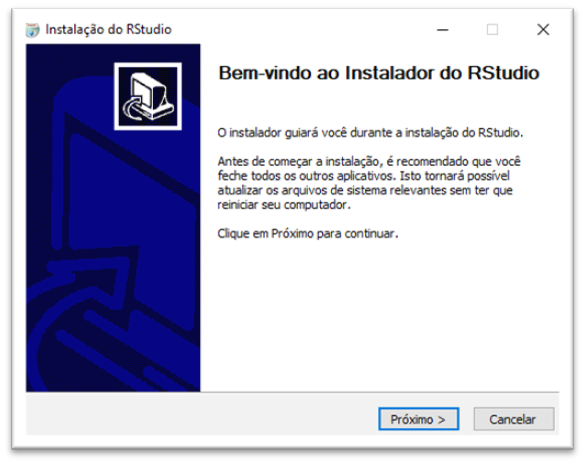
\includegraphics{images/clipboard-987499479.png}
  \end{center}
\end{enumerate}

Ao final da instalação, você deverá ser capaz de abrir o RStudio no seu
computador, resultando em algo similar à imagem abaixo. No Windows,
provavelmente você o encontrará no caminho:

\texttt{C:\textbackslash{}ProgramData\textbackslash{}Microsoft\textbackslash{}Windows\textbackslash{}Start\ Menu\textbackslash{}Programs\textbackslash{}RStudio}

\begin{center}
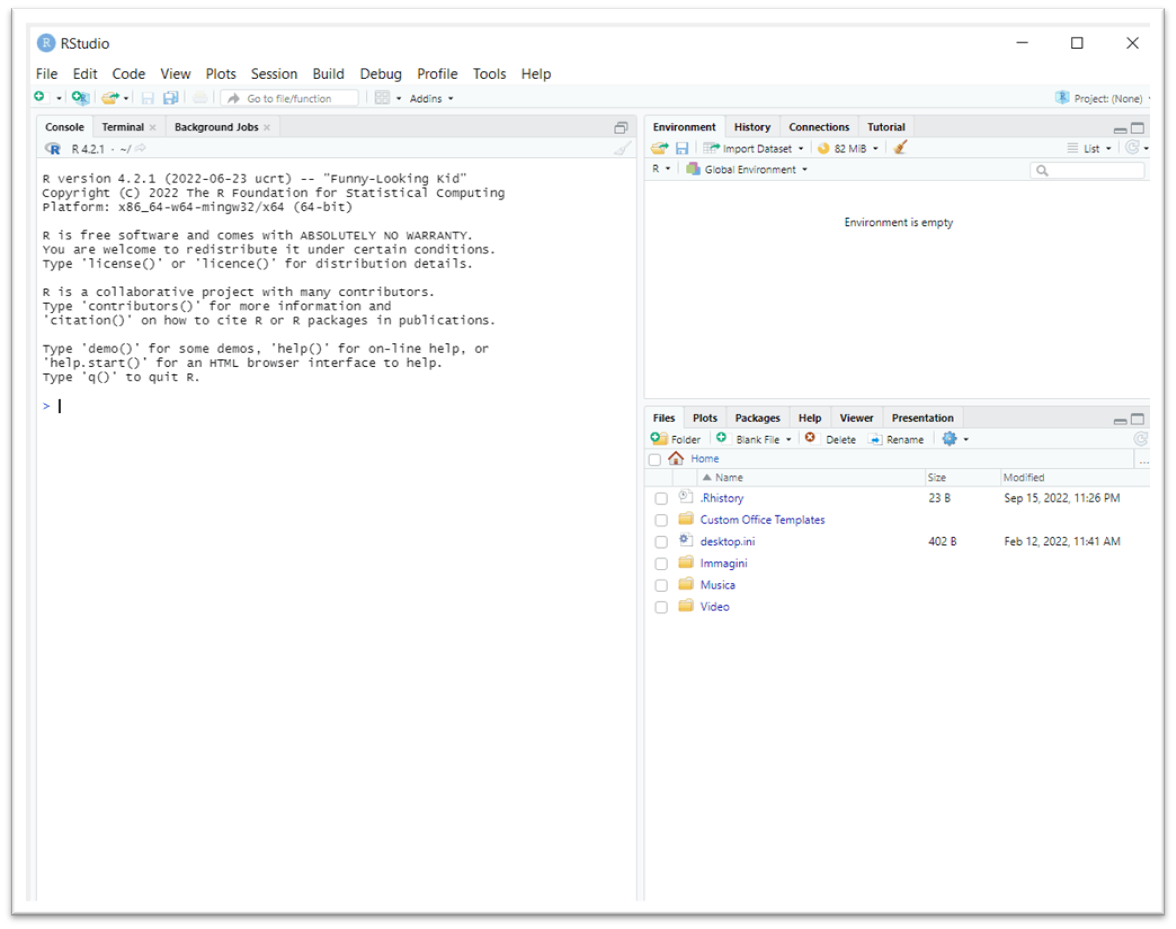
\includegraphics{images/clipboard-1128946571.png}
\end{center}

\textbf{Feito? Então estamos prontos para utilizar o R através do
RStudio!}

\section{Conhecendo o RStudio}\label{conhecendo-o-rstudio}

\begin{tcolorbox}[enhanced jigsaw, colback=white, colframe=quarto-callout-note-color-frame, colbacktitle=quarto-callout-note-color!10!white, bottomrule=.15mm, opacityback=0, breakable, opacitybacktitle=0.6, left=2mm, titlerule=0mm, toptitle=1mm, bottomtitle=1mm, arc=.35mm, title=\textcolor{quarto-callout-note-color}{\faInfo}\hspace{0.5em}{Nota}, rightrule=.15mm, toprule=.15mm, leftrule=.75mm, coltitle=black]

A seção 3.2 `Conhecendo o RStudio' é baseada na seção
\href{https://livro.curso-r.com/2-1-telas.html}{2.1 `Telas'} do livro
\emph{Ciência de Dados em R}, feito pelo Curso-R. De qualquer modo,
eventuais erros são inteiramente de nossa responsabilidade.

\end{tcolorbox}

O RStudio será o ambiente no qual iremos trabalhar com a linguagem. Por
essa razão, é \emph{muito} importante que você se sinta confortável com
o que verá no seu computador após abrí-lo. Nessa seção, iremos
compreender melhor o \emph{layout} do RStudio, além das utilidades que
ele nos proporciona ao longo do processo de escrita dos códigos.

Ao abrir o RStudio pela primeira vez (como na imagem anterior), você
verá inicialmente 3 quadrantes. Um deles, preenchendo a parte esquerda
da tela, já conhecemos: é o \textbf{Console}, que cumpre o mesmo papel
explicado no capítulo anterior. Ao mesmo tempo, o quadrante que mais
utilizaremos não aparece inicialmente: é o \textbf{Editor de Código},
outro velho conhecido que também possui a mesma atribuição anterior. Tal
como no caso do RGui, o Editor não abre automaticamente pois o RStudio
não é capaz de saber se o usuário tem o desejo de construir um código do
zero -- ou seja, criar um novo arquivo com extensão \emph{.R} -- ou
apenas dar continuidade à algum em que já estava trabalhando.

No fim das contas, teremos 4 quadrantes:

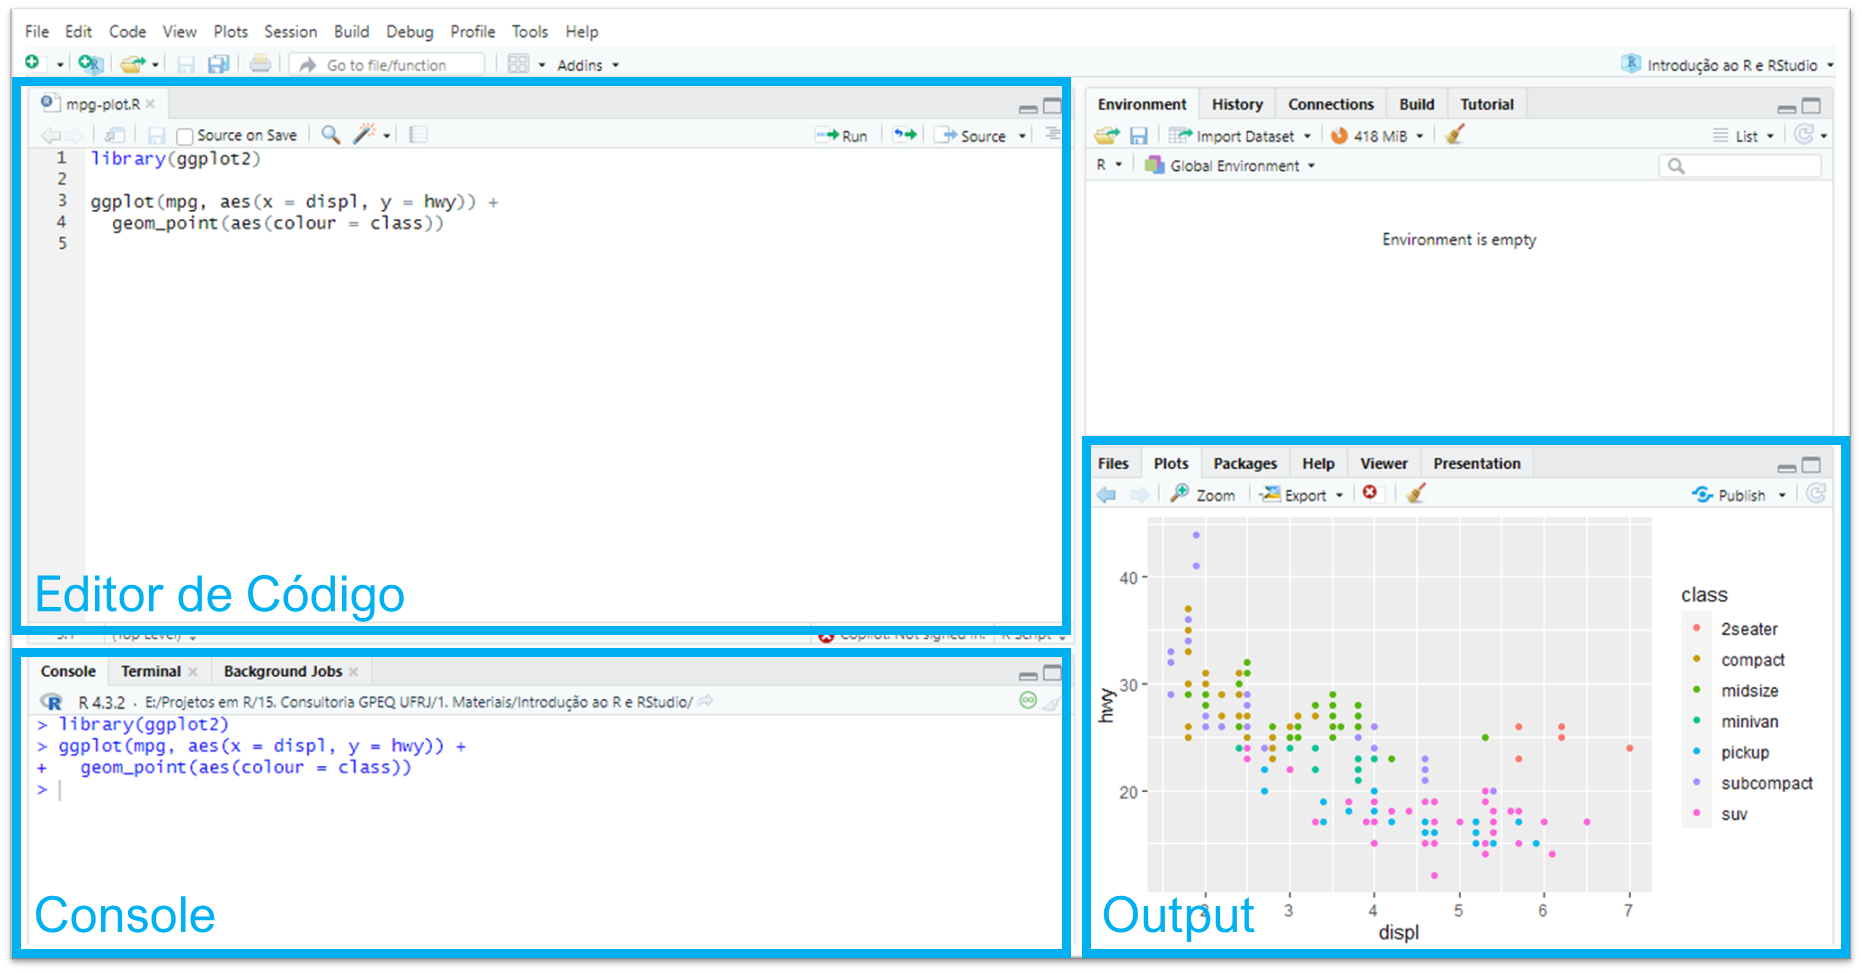
\includegraphics{images/clipboard-1486032127.png}

\begin{tcolorbox}[enhanced jigsaw, left=2mm, arc=.35mm, colback=white, rightrule=.15mm, colframe=quarto-callout-note-color-frame, leftrule=.75mm, bottomrule=.15mm, opacityback=0, toprule=.15mm, breakable]
\begin{minipage}[t]{5.5mm}
\textcolor{quarto-callout-note-color}{\faInfo}
\end{minipage}%
\begin{minipage}[t]{\textwidth - 5.5mm}

Por padrão, os quadrantes estarão dispostos na sua tela da forma como
mostramos na imagem acima, mas você pode organizá-los da forma que
preferir acessando a seção \emph{Pane Layout} da opção
\texttt{Global\ options...} no menu \texttt{Tools}.

\end{minipage}%
\end{tcolorbox}

É importante que você entenda que o Editor e o Console são os dois
principais quadrantes do RStudio. Passaremos a maior parte do tempo
neles. Como não custa nada, vamos relembrar suas respectivas serventias:

\begin{itemize}
\item
  \textbf{Editor de Código}: é local em que escreveremos/editaremos
  nossos códigos, salvando posteriormente em um arquivo do tipo
  \texttt{.R}. Conforme formos avançando, você acabará reparando que
  temos algumas melhorias em relação ao RGui:

  \begin{enumerate}
  \def\labelenumi{\arabic{enumi}.}
  \tightlist
  \item
    O RStudio colore algumas palavras e símbolos para \emph{facilitar} a
    leitura do código. Por exemplo, tudo o que for comentário será de
    uma determinada cor, assim como tudo que você escrever entre aspas
    -- considerado texto passível de ser executado como parte de um
    código -- será de outra.
  \item
    Outra funcionalidade interessante do Editor no RStudio é a
    capacidade de você poder buscar e substituir determinadas
    palavras/expressões que estejam presentes no código, poupando tempo
    e evitando erros caso o fizessemos de forma maunal; para tal, basta
    clicar no símbolo da lupa logo acima da primeira linha.
  \item
    Além disso, o RStudio possui o recurso de autocompletar partes de um
    código! Caso você esteja escrevendo o nome de um \emph{objeto} que
    ele consiga identificar, receberá automaticamente uma sugestão para
    completar a escrita, bastando apertar a tecla \texttt{Tab} para
    aceitá-la.
  \end{enumerate}
\item
  \textbf{Console}: é local em que o código é executado e recebemos as
  saídas. Nele, temos também o recurso de autocompletar nomes de
  objetos. Para \emph{limpar} o Console, isto é, excluir o registro do
  que já foi executado pelo R, basta clicar no símbolo de vassoura, no
  canto direito superior do quadrante, ou então utilizar o atalho
  \texttt{Ctrl\ +\ L}.
\end{itemize}

Os demais quadrantes do lado \emph{direito} contém painéis auxiliares. O
objetivo deles é facilitar pequenas tarefas que fazem parte tanto da
programação quanto da análise de dados como, por exemplo, olhar a
documentação de funções, analisar os objetos criados em uma sessão do R,
procurar e organizar os arquivos que compõem a nossa análise, armazenar
e analisar os gráficos criados e muito mais.

No quadrante \emph{superior}, temos

\begin{itemize}
\item
  \textbf{Environment}: painel com todos os objetos criados na sessão.
  Será bastante útil como referência para avaliar os objetos que criamos
  ou deixamos de criar com determinado comando.
\item
  \textbf{History}: painel com um histórico dos comandos rodados.
\end{itemize}

Já no quadrante \emph{inferior}, temos

\begin{itemize}
\item
  \textbf{Files}: mostra os arquivos no diretório de trabalho. Nele, é
  possível navegar entre as pastas do seu computador! Você pode, por
  exemplo, abrir um arquivo do tipo \texttt{.R} sem necessariamente ter
  que passar pela janela de busca do seu sistema operacional.
\item
  \textbf{Plots}: painel onde os gráficos serão apresentados, caso você
  crie um código que os produza.
\item
  \textbf{Packages}: apresenta todos os pacotes instalados e carregados.
\item
  \textbf{Help}: janela onde as documentações de funções serão
  apresentadas.
\item
  \textbf{Viewer}: painel onde relatórios e dashboards serão
  apresentados.
\end{itemize}

Além do Console e do Editor, dê atenção especial aos painéis
Environment, Help e Plots, nesta ordem.

\part{Programando em R}

Nessa parte do material, você aprenderá a programar na prática. O
capítulo inicial terá como objetivo estimular que a escrita de suas
primeiras linhas de código; será composto de tarefas \emph{super}
simples, mas suficientes para proporcionar uma primeira eperiência à
quem nunca programou. Nos dois capítulos seguintes, te guiaremos no
entendimento sobre os dois conceitos mais importantes da linguagem:
\emph{objetos} e \emph{funções}. Segundo John Chambers, um dos
desenvolvedores do R,

\begin{quote}
\emph{to understand computations in R, two slogans are helpful:}

\begin{itemize}
\item
  \emph{Everything that exists is an object.}
\item
  \emph{Everything that happens is a function call.}
\end{itemize}
\end{quote}

O último capítulo, por sua vez, te ensinará a como armazenar informações
externas no R. É importante que você saiba esse tópico pois, em algumas
matérias, seu professor lhe entregará arquivos com informações nos quais
algumas tarefas deverão ser executadas com auxílio da linguagem.

\chapter{Primeiros passos}\label{primeiros-passos}

\begin{tcolorbox}[enhanced jigsaw, left=2mm, arc=.35mm, colback=white, rightrule=.15mm, colframe=quarto-callout-note-color-frame, leftrule=.75mm, bottomrule=.15mm, opacityback=0, toprule=.15mm, breakable]

Partes deste capítulo são baseadas na seção
\href{https://livro.curso-r.com/3-2-r-como-calculadora.html}{3.2 `R como
calculadora'} do livro \emph{Ciência de Dados em R}, feito pelo Curso-R.
De qualquer modo, eventuais erros são inteiramente de nossa
responsabilidade.

\end{tcolorbox}

Como vimos nos capítulos anteriores, o papel do \textbf{Console} no R é
interpretar os nossos comandos à luz da linguagem. Ele avalia o código
que o passamos e devolve a saída correspondente --- se tudo der certo
--- ou uma mensagem de erro --- se o seu código tiver algum problema.
Essa operação é chamada de \textbf{avaliar}, \textbf{executar} ou
\textbf{rodar} o código. Para que seu código seja executado diretamente
no Console, escreva-o e, na sequência, aperte \texttt{Enter}. A outra
forma de executar uma expressão é escrever o código em um \emph{script}
no \textbf{Editor}, deixar o cursor em cima da linha e usar o atalho
\texttt{Ctrl\ +\ Enter}. Assim, o comando é enviado para o Console, onde
é diretamente executado.

Nesse capítulo, você \emph{rodará} suas primeiras linhas de código com
intuito de realizar operações aritméticas como \emph{adição},
\emph{subtração}, \emph{multiplicação} e \emph{divisão}, além de
comparações lógicas simples. O objetivo aqui não é te ensinar matemática
básica, mas te preparar para a execução de linhas de código mais
avançadas. É a forma mais fácil de um iniciante ganhar familiaridade e
experiência prática com o R.

\section{Operadores Aritméticos}\label{operadores-aritmuxe9ticos}

De agora em diante, cada região sombreada de cinza representa código, ao
passo que seu resultado estará exposto logo na sequência. Vamos começar
com um exemplo simples:

\begin{Shaded}
\begin{Highlighting}[]
\DecValTok{1} \SpecialCharTok{+} \DecValTok{1}
\end{Highlighting}
\end{Shaded}

\begin{verbatim}
[1] 2
\end{verbatim}

Nesse caso, o nosso comando foi o código \texttt{1\ +\ 1} e a saída foi
o valor \texttt{2}. Como você pode reproduzir esse comando no RStudio?
Inicialmente, copie o que está escrito acima ao clicar no símbolo de
prancheta no canto superior direito da região sombreada. Na sequência,
cole no Editor de Código e aperte \texttt{Ctrl\ +\ Enter} (ou então no
Console, pressionando apenas \texttt{Enter}). Observe abaixo!

\begin{center}
\includegraphics{images/1mais1.gif}
\end{center}

Tente agora jogar no Console a expressão:
\texttt{2\ *\ 2\ -\ (4\ +\ 4)\ /\ 2}. Deu zero? Pronto! Você já é capaz
de pedir ao R para fazer \emph{qualquer uma das quatro operações
aritméticas básicas}. Repare que as operações e suas precedências são
mantidas como na matemática, ou seja, divisão e multiplicação são
calculadas antes da adição e subtração, além de os parênteses ditarem a
ordem na qual serão realizadas. A seguir, apresentamos a
Tabela~\ref{tbl-ope-mat} resumindo como fazer as principais operações no
R.

\begin{longtable}[]{@{}cccc@{}}

\caption{\label{tbl-ope-mat}Operadores matemáticos do R}

\tabularnewline

\toprule\noalign{}
Operação & Operador & Exemplo & Resultado \\
\midrule\noalign{}
\endhead
\bottomrule\noalign{}
\endlastfoot
Adição & + & 1 + 1 & 2.00 \\
Subtração & - & 4 - 2 & 2.00 \\
Multiplicação & * & 2 * 3 & 6.00 \\
Divisão & / & 5 / 3 & 1.67 \\
Potenciação & \^{} & 4 \^{} 2 & 16.00 \\
Resto da Divisão & \%\% & 5 \%\% 3 & 2.00 \\
Parte Inteira da Divisão & \%/\% & 5 \%/\% 3 & 1.00 \\

\end{longtable}

\section{Operadores Lógicos}\label{operadores-luxf3gicos}

O R permite também testar comparações lógicas. Os valores lógicos
básicos em R são \texttt{TRUE} (ou apenas \texttt{T}) e \texttt{FALSE}
(ou apenas \texttt{F}). Por exemplo, podemos pedir ao R que nos diga se
é verdadeiro que 5 é menor do que 3. Como a resposta é obviamente
negativa, ele retornará \texttt{FALSE}, nos dizendo que a proposição que
fizemos é falsa.

\begin{Shaded}
\begin{Highlighting}[]
\DecValTok{5} \SpecialCharTok{\textless{}} \DecValTok{3}
\end{Highlighting}
\end{Shaded}

\begin{verbatim}
[1] FALSE
\end{verbatim}

Abaixo, introduzimos a Tabela~\ref{tbl-ope-log} com outros operadores
lógicos da linguagem.

\begin{longtable}[]{@{}
  >{\centering\arraybackslash}p{(\columnwidth - 6\tabcolsep) * \real{0.2151}}
  >{\centering\arraybackslash}p{(\columnwidth - 6\tabcolsep) * \real{0.1075}}
  >{\centering\arraybackslash}p{(\columnwidth - 6\tabcolsep) * \real{0.5591}}
  >{\centering\arraybackslash}p{(\columnwidth - 6\tabcolsep) * \real{0.1183}}@{}}

\caption{\label{tbl-ope-log}Operadores lógicos do R}

\tabularnewline

\toprule\noalign{}
\begin{minipage}[b]{\linewidth}\centering
Operação
\end{minipage} & \begin{minipage}[b]{\linewidth}\centering
Operador
\end{minipage} & \begin{minipage}[b]{\linewidth}\centering
Exemplo
\end{minipage} & \begin{minipage}[b]{\linewidth}\centering
Resultado
\end{minipage} \\
\midrule\noalign{}
\endhead
\bottomrule\noalign{}
\endlastfoot
Maior que & \textgreater{} & 2 \textgreater{} 1 & TRUE \\
Maior ou igual que & \textgreater= & 2 \textgreater= 2 & TRUE \\
Menor que & \textless{} & 2 \textless{} 3 & TRUE \\
Menor ou igual que & \textless= & 5 =\textless{} 3 & FALSE \\
Igual à & == & 4 == 4 & TRUE \\
Diferente de & != & 5 != 3 & TRUE \\
x \textbf{e} y & \& & x \textless- c(1, 4, NA, 8) x{[}!is.na(x) \& x
\textgreater{} 5{]} & 8 \\
x \textbf{ou} y & \textbar{} & x \textless- c(1, 4, NA, 8) x{[}!is.na(x)
\textbar{} x \textgreater{} 5{]} & 1, 4, 8 \\

\end{longtable}

\section{Possíveis complicações}\label{possuxedveis-complicauxe7uxf5es}

Se você digitar um comando incompleto, como \texttt{5\ +}, e apertar
\texttt{Enter}, o R mostrará um \texttt{+}, o que não tem nada a ver com
a adição da matemática. Isso significa que o R está esperando você
enviar \textbf{mais} algum código para completar o seu comando. Termine
o seu comando ou aperte \texttt{Esc} para recomeçar.

\begin{Shaded}
\begin{Highlighting}[]
\DecValTok{5} \SpecialCharTok{{-}}
\SpecialCharTok{+} 
\SpecialCharTok{+} \DecValTok{5}
\end{Highlighting}
\end{Shaded}

\begin{verbatim}
[1] 0
\end{verbatim}

Se você digitar um comando que o R não reconhece, ele retornará uma
mensagem de erro. \textbf{Não entre em pânico.} Ele só está te avisando
que não conseguiu interpretar o comando.

\begin{Shaded}
\begin{Highlighting}[]
\DecValTok{5}\NormalTok{ \% }\DecValTok{2}
\end{Highlighting}
\end{Shaded}

\begin{verbatim}
Error: <text>:1:3: unexpected input
1: 5 % 2
      ^
\end{verbatim}

Você pode digitar outro comando normalmente em seguida.

\begin{Shaded}
\begin{Highlighting}[]
\DecValTok{5} \SpecialCharTok{\^{}} \DecValTok{2}
\end{Highlighting}
\end{Shaded}

\begin{verbatim}
[1] 25
\end{verbatim}

\chapter{Objetos}\label{objetos}

Na apresentação dessa parte do material, trouxemos uma citação que, em
parte, dizia:

\begin{quote}
\textbf{\emph{Everything that exists is an object.}}
\end{quote}

\textbf{Um objeto é simplesmente um nome que guarda um valor ou código.}
Não há como ser mais direto: tudo que existe no R é um \emph{objeto,
inclusive as funções que veremos no capítulo seguinte}. Nesse capítulo,
veremos com detalhe os objetos que são designados à \emph{armazenar
dados}. Antes, no entanto, vamos dar um passo para trás e explicar o que
são dados.

\section{Dados}\label{dados}

Segundo a Oxford Languages, dados são

\begin{quote}
fatos e estatísticas coletadas de forma conjunta para referência ou
análise.
\end{quote}

\textbf{Na prática, dados nos mostram informações sobre determinado
indivíduo ou situação que procuramos descrever, seja uma pessoa,
instituição, comportamento, condição geográfica, etc.} O número de horas
que você dormiu essa noite é um dado. A lista que relata quem é ou não
calvo na sua família é uma \emph{coleção} de dados. A expectativa, hoje,
de quanto será a inflação acumulada nos próximos 12 meses é um dado. A
variação percentual do Produto Interno Bruto (PIB) real no último
trimestre é um dado. A lista que mostra a sequência de variações do PIB
real nos últimos dez trimestres é uma \emph{série temporal}, isto é,
dados em sequência ao longo do tempo.

\subsection{Tipo \& Forma}\label{tipo-forma}

Vamos nos aprofundar um pouco mais. Ao lidar formalmente com dados,
\textbf{devemos ter mente que eles são compostos por uma ou mais
variáveis e seus valores}. \emph{Uma variável é uma dimensão ou
propriedade que descreve uma unidade de observação} (por exemplo, uma
pessoa) e normalmente pode assumir valores diferentes. Por outro lado,
os \emph{valores são as instâncias concretas que uma variável atribui a
cada unidade de observação e são ainda caracterizados por seu intervalo}
(por exemplo, valores categóricos versus valores contínuos) \emph{e seu
tipo} (por exemplo, valores lógicos, numéricos ou de caracteres).
Estaremos interessados no \emph{tipo} dos dados. A
Tabela~\ref{tbl-data-types} apresenta os que podem aparecer com maior
frequência.

\begin{longtable}[]{@{}
  >{\centering\arraybackslash}p{(\columnwidth - 4\tabcolsep) * \real{0.1935}}
  >{\centering\arraybackslash}p{(\columnwidth - 4\tabcolsep) * \real{0.6129}}
  >{\centering\arraybackslash}p{(\columnwidth - 4\tabcolsep) * \real{0.1935}}@{}}

\caption{\label{tbl-data-types}Tipos mais comuns de dados}

\tabularnewline

\toprule\noalign{}
\begin{minipage}[b]{\linewidth}\centering
Tipo
\end{minipage} & \begin{minipage}[b]{\linewidth}\centering
Serve para representar\ldots{}
\end{minipage} & \begin{minipage}[b]{\linewidth}\centering
Exemplo
\end{minipage} \\
\midrule\noalign{}
\endhead
\bottomrule\noalign{}
\endlastfoot
Númerico & números do tipo \emph{integer} (inteiro) ou \emph{double}
(reais) & 1, 3.2, 0.89 \\
Texto \emph{(string)} & caracteres (letras, palavras ou setenças) &
``Ana jogou bola'' \\
Lógico & valores verdade do tipo lógico (valores booleanos) & TRUE,
FALSE, NA \\
Tempo & datas e horas & 14/04/1999 \\

\end{longtable}

Voltando ao primeiro exemplo, uma pessoa pode ser descrita pelas
variáveis \emph{nome}, \emph{número de horas dormidas} e \emph{se dormiu
ou não mais de oito horas}. Os valores correspondentes a essas variáveis
seriam do tipo texto (por exemplo, ``Pedro''), numéricos (número de
horas) e lógicos (\texttt{TRUE} ou \texttt{FALSE}, definido em função do
tempo descansado\footnote{Se o número de horas que a pessoa descansou
  for maior do que 8, então a variável deverá apresentar valor igual a
  \texttt{TRUE} -- ou seja, é verdade que a pessoa dormiu mais de 8
  horas. Caso contrário, \texttt{FALSE}.}). \textbf{Note a diferença
entre \emph{dado} e \emph{valor}.} O número 10 é um valor, sem
significado. Por outro lado, \emph{``10 horas dormidas''} é um dado,
caracterizado pelo valor 10 e pela variável \emph{``horas dormidas''}.

Outro aspecto importante sobre os dados está em sua forma, ou seja, como
os dados podem ser organizados. A Tabela~\ref{tbl-data-shapes} apresenta
as formas mais comuns de organização.

\begin{longtable}[]{@{}
  >{\centering\arraybackslash}p{(\columnwidth - 4\tabcolsep) * \real{0.1758}}
  >{\centering\arraybackslash}p{(\columnwidth - 4\tabcolsep) * \real{0.5165}}
  >{\centering\arraybackslash}p{(\columnwidth - 4\tabcolsep) * \real{0.3077}}@{}}

\caption{\label{tbl-data-shapes}Formas pelas quais os dados podem ser
organizados}

\tabularnewline

\toprule\noalign{}
\begin{minipage}[b]{\linewidth}\centering
Formato
\end{minipage} & \begin{minipage}[b]{\linewidth}\centering
Os dados se apresentam como\ldots{}
\end{minipage} & \begin{minipage}[b]{\linewidth}\centering
Exemplo
\end{minipage} \\
\midrule\noalign{}
\endhead
\bottomrule\noalign{}
\endlastfoot
Escalar & elementos individuais & ``AB'', 4, TRUE \\
Retangular & dados organizados em \(i\) linhas e \(j\) colunas & Vetores
e Tabelas de Dados \\
Não-retangular & junção de uma ou mais estruturas de dados & Listas \\

\end{longtable}

Um escalar é um elemento único, que pode ser de qualquer tipo. Ou seja,
a representação elementar de um dado se dá através de um escalar! Por
exemplo, o tipo sanguíneo de determinada pessoa, representado pelos
caracteres ``AB'', é um escalar do tipo texto. Você pode pensar no
escalar como um dado organizado em 1 linha e 1 coluna.

Por sua vez, dados retangulares são àqueles cuja organização ocorre em
\(i\) linhas e \(j\) colunas, tal que \(i,j \in \mathbb{N}\) e \(i > 1\)
ou \(j > 1\). As formas retangulares mais comuns são \emph{vetores},
\emph{matrizes} e \emph{tabelas de dados}. Uma matriz é uma forma de
organização de dados \emph{númericos} em em \(i\) linhas e \(j\)
colunas. Quando uma matriz possui \(i\) linhas e \(1\) coluna \emph{ou}
\(1\) linha e \(j\) colunas, chamamos de vetor-coluna e vetor-linha,
respectivamente; em muitos casos, chamamos apenas de \emph{vetor}.
Assim, o vetor é um caso especial de matriz unidimensional. As tabelas
de dados, por outro lado, possuem \(i\) linhas e \(j\) colunas, tal que
\(i > 1\) e \(j > 1\). Além disso, aceitam todos os tipos de dado -- por
exemplo, númericos, de textos ou lógicos -- em qualquer que seja a
combinação de linha e coluna.

Por sua vez, dados não-retangulares se referem a toda organização de
dados que não seja feita em linhas e colunas relacionadas entre si. A
forma mais comum é a lista. Observe um exemplo abaixo: cada
característica pode ser entendida como um elemento de uma lista. Apesar
de pertencerem a mesma estrutura, os elementos não se comunicam entre
si.

\begin{longtable}[]{@{}llllll@{}}
\toprule\noalign{}
\endhead
\bottomrule\noalign{}
\endlastfoot
~ & ~ & ~ & ~ & ~ & ~ \\
~ & Jorge & Laís & Matheus & Laura & Nathália \\
Gênero & Masculino & Feminino & Masculino & Feminino & Feminino \\
~ & ~ & ~ & ~ & ~ & ~ \\
~ & Jorge & Laís & Matheus & Laura & Nathália \\
Idade & 18 & 23 & 22 & 21 & 21 \\
~ & ~ & ~ & ~ & ~ & ~ \\
~ & Jorge & Laís & Matheus & Laura & Nathália \\
Altura (cm) & 180 & 170 & 170 & 175 & 168 \\
~ & ~ & ~ & ~ & ~ & ~ \\
~ & Jorge & Laís & Matheus & Laura & Nathália \\
Peso (kg) & 76 & 65 & 70 & 68 & 66 \\
~ & ~ & ~ & ~ & ~ & ~ \\
\end{longtable}

Nesse caso em específico, conseguimos fazer a transição para uma tabela
(forma retangular) pois todos os elementos são são características das
mesmas pessoas. Em uma tabela de dados, automaticamente temos uma
relação entre os dados: cada linha contém características de uma unidade
específica.

\captionsetup{labelsep=none}

\begin{longtable}[]{@{}ccccc@{}}

\caption{\label{tbl-tabela-retangular}}

\tabularnewline

\toprule\noalign{}
Nome & Gênero & Idade & Altura (cm) & Peso (kg) \\
\midrule\noalign{}
\endhead
\bottomrule\noalign{}
\endlastfoot
Jorge & Masculino & 18 & 180 & 76 \\
Laís & Feminino & 23 & 170 & 65 \\
Matheus & Masculino & 22 & 175 & 70 \\
Laura & Feminino & 21 & 181 & 68 \\
Nathália & Feminino & 21 & 168 & 66 \\

\end{longtable}

\section{Estruturas de Dados no R}\label{estruturas-de-dados-no-r}

Na seção anterior, vimos os conceitos de \emph{tipo} e \emph{forma}.
Tenha em mente que são duas definições que existem independentemente de
qualquer linguagem de programação -- elas versam sobre \emph{dados} de
forma geral.

Por outro lado, agora veremos o conceito e alguns exemplos de
\emph{estrutura de dados} para o R. \textbf{A estrutura de dados é a
forma pela qual o R classificará um objeto em relação ao \emph{tipo} e a
\emph{forma} dos dados que contém.} Existe uma estrutura de dados para
cada combinação de tipo e forma? \textbf{Não.} Compreender as principais
estruturas disponíveis no R requer vê-las como uma combinação de

\begin{enumerate}
\def\labelenumi{(\alph{enumi})}
\tightlist
\item
  \emph{algum} formato de dados
\item
  o fato de conterem um único ou vários tipos de dados
\end{enumerate}

\subsection{Criando e armazenando objetos na
memória}\label{criando-e-armazenando-objetos-na-memuxf3ria}

Antes de conhecê-las, no entanto, vamos entender melhor os comandos para
criar e armazenar \emph{qualquer} objeto (seja ele para armazenar dados,
como nesse capítulo, ou para criar funções, que serão vistas no próximo)
na memória do R.

Para \emph{criar} e \emph{armazenar} um objeto, sempre escreveremos
inicialmente seu nome (escolhido por você), seguido de um dos
\emph{operadores} \emph{de atribuição} (ou \emph{assingment operators},
como são conhecidos) e, por fim, o objeto propriamente dito com as
informações de nosso interesse. O principal operador de atribuição para
se criar objetos é \texttt{\textless{}-}. Outro operador que é comumente
utilizado para cumprir a mesma tarefa é \texttt{=}. Ainda que exista uma
leve diferença entre ambos, ao longo dos cursos será possível utilizar o
operador de sua preferência. Por ser o ideal, utilizaremos
\texttt{\textless{}-} no restante do material.

\begin{Shaded}
\begin{Highlighting}[]
\NormalTok{nome\_do\_objeto }\OtherTok{\textless{}{-}} \ErrorTok{\textgreater{}}\NormalTok{objeto com informações}\SpecialCharTok{\textless{}}
  
\NormalTok{nome do objeto }\OtherTok{=}  \ErrorTok{\textgreater{}}\NormalTok{objeto com informações}\SpecialCharTok{\textless{}}
\end{Highlighting}
\end{Shaded}

No parágrafo anterior, observe que está escrito \emph{`criar e
armazenar'}. Nós poderíamos simplesmente criar um objeto, sem
armazená-lo na memória do R. Nesse caso, não teríamos o nome do objeto
disponível na aba \textbf{Environment} (ou seja, ele não seria
armazenado no nosso ambiente de trabalho) e seria bem mais complicado
registrar todas as mudanças que viermos a fazer nele. Aconteceria apenas
a ocorrência de uma única saída no Console com a estrutura do objeto
criado (de forma semelhante ao que fizemos no capítulo anterior) -- o
quê não tem grande utilidade para nós, exceto caso você queira verificar
a estrutura do objeto antes de realmente armazená-lo.

Ao mesmo tempo, você irá perceber que a \emph{criação e armazenamento de
um objeto não implica sua visualização imediata}. Isso signfinica que,
ao dar o comando para criar algum objeto, não acontecerá nada no
Console. Você pode acabar achando que o processo falhou ou algo do tipo,
mas não é nada disso! Como dissemos, a mudança ocorrerá na aba
Environment, onde deverá aparecer o nome do novo objeto. Para visualizar
o objeto criado, escreva seu nome e rode a linha de código. Agora sim o
objeto aparecerá no Console.

\begin{Shaded}
\begin{Highlighting}[]
\NormalTok{nome\_do\_objeto}
\end{Highlighting}
\end{Shaded}

Se você criou e armazenou um objeto na memória, ele ficará por lá até
que você encerre sua sessão atual (feche o RStudio) ou, então, que o
remova. Para remover qualquer objeto basta escrever
\texttt{rm(nome\_do\_objeto)}. Caso tenha o desejo de remover vários
objetos, basta separar seus nomes com vírgula. Para remover \emph{todos}
os objetos que aparecem na aba Environment, use
\texttt{rm(list\ =\ ls())}.

\begin{Shaded}
\begin{Highlighting}[]
\FunctionTok{rm}\NormalTok{(nome\_do\_objeto1)}

\FunctionTok{rm}\NormalTok{(nome\_do\_objeto1, nome\_do\_objeto2, ...)}

\FunctionTok{rm}\NormalTok{(}\AttributeTok{list =} \FunctionTok{ls}\NormalTok{())}
\end{Highlighting}
\end{Shaded}

Observe no GIF abaixo como é na prática!

\begin{center}
\includegraphics[width=6.45833in,height=\textheight]{images/criando_objeto.gif}
\end{center}

\subsection{Valor único}\label{valor-uxfanico}

Ao criar um objeto com valor único, estamos armazenando um escalar que
pode variar quanto ao tipo (por exemplo, númerico, \emph{string} ou
valor lógico). Nesse caso, a \emph{estrutura} do objeto \emph{será
idêntica} ao \emph{tipo} -- o que faz sentido, afinal estamos falando de
um objeto de uma única linha e coluna.

\subsubsection{Numérico}\label{numuxe9rico}

Um objeto \textbf{númerico} contém apenas um número (por exemplo, 1, 2,
4.13, \(\pi\), entre outros). Se quisessemos atribuir o valor numérico 5
à um objeto chamado \texttt{x}, como poderiamos fazer? Observe abaixo e
replique no seu RStudio!

\begin{Shaded}
\begin{Highlighting}[]
\NormalTok{x }\OtherTok{\textless{}{-}} \DecValTok{5} 
\end{Highlighting}
\end{Shaded}

Note que o Console não retorna nenhuma mensagem ou valor. Como dissemos
na seção anterior, a única diferença que você deve ser capaz de observar
é no painel Environment, no quadrante superior direito do RStudio. O
nome do novo objeto aparecerá lá. Para que você possa visualizar o
conteúdo do objeto criado, terá que escrever apenas seu nome e rodar a
linha de código!

\begin{Shaded}
\begin{Highlighting}[]
\NormalTok{x}
\end{Highlighting}
\end{Shaded}

\begin{verbatim}
[1] 5
\end{verbatim}

\subsubsection{Textual}\label{textual}

Uma \textbf{sequência de caracteres} (\emph{character string}, ou apenas
\emph{string}) é um conjunto de caracteres dentro de um par de aspas e
pode ou não incluir espaços. Por exemplo, ``elevada'' e ``pressão
arterial elevada'' são objetos de caracteres com um único valor de
\emph{string}.

\begin{Shaded}
\begin{Highlighting}[]
\NormalTok{y }\OtherTok{\textless{}{-}} \StringTok{"pressão arterial elevada"} 
\NormalTok{y}
\end{Highlighting}
\end{Shaded}

\begin{verbatim}
[1] "pressão arterial elevada"
\end{verbatim}

\subsection{Vetor}\label{vetor}

Um \textbf{vetor} contém uma coleção ordenada de dados indexados pelos
inteiros \(1, 2,..., n\), onde \(n\) é o comprimento do vetor. \emph{O
vetor como estrutura de dados é a combinação da forma vetor com dados de
um único tipo, não necessariamente numérico.} No exemplo abaixo, um
vetor númerico, isto é, que contém apenas números.

\begin{Shaded}
\begin{Highlighting}[]
\NormalTok{z }\OtherTok{\textless{}{-}} \FunctionTok{c}\NormalTok{(}\DecValTok{5}\NormalTok{, }\DecValTok{8}\NormalTok{, }\DecValTok{12}\NormalTok{) }
\NormalTok{z}
\end{Highlighting}
\end{Shaded}

\begin{verbatim}
[1]  5  8 12
\end{verbatim}

\textbf{Se você tentar criar um vetor contendo dois tipos de dados
diferentes, ele converterá todos os dados para o tipo texto.} A única
exceção é com relação a entradas do tipo lógico \texttt{NA} \emph{(Not
Available)}, que representam a ausência de determinado dado.

\begin{Shaded}
\begin{Highlighting}[]
\NormalTok{z }\OtherTok{\textless{}{-}} \FunctionTok{c}\NormalTok{(}\DecValTok{5}\NormalTok{, }\StringTok{"texto"}\NormalTok{, }\ConstantTok{TRUE}\NormalTok{, }\ConstantTok{NA}\NormalTok{)}
\NormalTok{z}
\end{Highlighting}
\end{Shaded}

\begin{verbatim}
[1] "5"     "texto" "TRUE"  NA     
\end{verbatim}

É inegável que, a partir deste ponto, as estruturas começam a ficar mais
interessantes. Lembre-se que o vetor tem uma dimensão e pode ter muitas
informações armazenadas. É natural que, em determinadas situações,
desejemos acessar apenas valores específicos dentre os que constam nele.

Como podemos fazer isso? Note que podemos associar a cada elemento de um
vetor um número, representando a linha ou coluna em que consta. A esse
número chamamos de índice! Dessa forma, fica fácil acessar qualquer um
de seus valores. Basta escrever, ao lado de seu nome e entre colchetes,
o índice que está associado à este valor. Por exemplo, vamos acessar o
segundo elemento do vetor \texttt{z} que acabamos de criar.

\begin{Shaded}
\begin{Highlighting}[]
\NormalTok{z[}\DecValTok{2}\NormalTok{] }\CommentTok{\# Acessando o segundo elemento de um vetor}
\end{Highlighting}
\end{Shaded}

\begin{verbatim}
[1] "texto"
\end{verbatim}

\begin{tcolorbox}[enhanced jigsaw, colback=white, colframe=quarto-callout-tip-color-frame, colbacktitle=quarto-callout-tip-color!10!white, bottomrule=.15mm, opacityback=0, breakable, opacitybacktitle=0.6, left=2mm, titlerule=0mm, toptitle=1mm, bottomtitle=1mm, arc=.35mm, title=\textcolor{quarto-callout-tip-color}{\faLightbulb}\hspace{0.5em}{Outras formas de criar vetores (Opcional)}, rightrule=.15mm, toprule=.15mm, leftrule=.75mm, coltitle=black]

\begin{Shaded}
\begin{Highlighting}[]
\DecValTok{1}\SpecialCharTok{:}\DecValTok{7}                \CommentTok{\# Criando uma sequência de números de 1 a 7}
\end{Highlighting}
\end{Shaded}

\begin{verbatim}
[1] 1 2 3 4 5 6 7
\end{verbatim}

\begin{Shaded}
\begin{Highlighting}[]
\FunctionTok{seq}\NormalTok{(}\DecValTok{2}\NormalTok{, }\DecValTok{10}\NormalTok{, }\AttributeTok{by =} \DecValTok{2}\NormalTok{) }\CommentTok{\# Criando um sequência de 2 a 10 pulando um número. }
\end{Highlighting}
\end{Shaded}

\begin{verbatim}
[1]  2  4  6  8 10
\end{verbatim}

\begin{Shaded}
\begin{Highlighting}[]
\FunctionTok{rep}\NormalTok{(}\DecValTok{3}\NormalTok{, }\DecValTok{5}\NormalTok{)          }\CommentTok{\# Repetindo o número 3, 5 vezes }
\end{Highlighting}
\end{Shaded}

\begin{verbatim}
[1] 3 3 3 3 3
\end{verbatim}

\begin{Shaded}
\begin{Highlighting}[]
\FunctionTok{rep}\NormalTok{(}\FunctionTok{c}\NormalTok{(}\DecValTok{1}\NormalTok{,}\DecValTok{2}\NormalTok{), }\DecValTok{3}\NormalTok{)     }\CommentTok{\# Repetindo o vetor (1,2), 3 vezes}
\end{Highlighting}
\end{Shaded}

\begin{verbatim}
[1] 1 2 1 2 1 2
\end{verbatim}

\end{tcolorbox}

\subsubsection{Fator}\label{fator}

Um \textbf{fator} é um tipo especial de vetor que contém valores
numéricos subjacentes \(1, 2,..., n\), mas cada um desses \(n\) valores
possui um rótulo de texto associado (que pode ou não ser o valor
numérico). Esses valores rotulados são os \textbf{níveis}
\emph{(levels)} do fator. Um uso comum de um fator é armazenar uma
variável categórica. \textbf{Depois de criar um vetor de fator com
níveis específicos, nenhum elemento desse vetor poderá assumir um valor
que não seja um de seus níveis pré-atribuídos.}

Você pode criar um fator a partir de um vetor de caracteres e o R
assumirá que os valores únicos são os rótulos dos níveis. Por exemplo,
no exemplo abaixo os níveis serão ``lento'', ``normal'' e ``rápido''.

\begin{Shaded}
\begin{Highlighting}[]
\NormalTok{y }\OtherTok{\textless{}{-}} \FunctionTok{factor}\NormalTok{(}\FunctionTok{c}\NormalTok{(}\StringTok{"super rápido"}\NormalTok{, }\StringTok{"super lento"}\NormalTok{, }\StringTok{"normal"}\NormalTok{, }\StringTok{"super rápido"}\NormalTok{, }\StringTok{"normal"}\NormalTok{))}
\NormalTok{y         }\CommentTok{\# Rodar o vetor de fator também irá retornar os níveis}
\end{Highlighting}
\end{Shaded}

\begin{verbatim}
[1] super rápido super lento  normal       super rápido normal      
Levels: normal super lento super rápido
\end{verbatim}

Se quiser alterar os rótulos, você pode fazê-lo atribuindo um novo valor
aos seus níveis. Por exemplo, suponha que queiramos que os rótulos sejam
maiúsculos.

\begin{Shaded}
\begin{Highlighting}[]
\FunctionTok{levels}\NormalTok{(y) }\OtherTok{\textless{}{-}} \FunctionTok{c}\NormalTok{(}\StringTok{"Super Rápido"}\NormalTok{, }\StringTok{"Normal"}\NormalTok{, }\StringTok{"Super Lento"}\NormalTok{) }
\FunctionTok{levels}\NormalTok{(y)}
\end{Highlighting}
\end{Shaded}

\begin{verbatim}
[1] "Super Rápido" "Normal"       "Super Lento" 
\end{verbatim}

Como alternativa, você pode atribuir novos rótulos de nível ao criar o
fator. Isso tem a vantagem adicional de permitir que você decida em que
ordem os níveis devem aparecer. Quando criamos o fator, R atribuiu
automaticamente os níveis pegando os valores exclusivos de \texttt{y} e
colocando-os em ordem alfabética. Por vários motivos (como criar um
gráfico de barras posteriormente), você pode querer que os níveis
estejam em uma ordem diferente. \textbf{Você pode especificar a ordem
dos níveis ao criar a variável, mas tome cuidado porque se você deixar
de fora um valor que aparece nos dados esse valor acabará definido como
ausente (}\texttt{NA}\textbf{)}.

No exemplo anterior, gostaríamos que a ordem fosse da velocidade menor
para o maior.

\begin{Shaded}
\begin{Highlighting}[]
\CommentTok{\# Enter ORIGINAL values in levels }
\CommentTok{\# Enter the NEW level labels in labels }
\CommentTok{\# Make sure the orderings of levels and labels correspond }
\NormalTok{y }\OtherTok{\textless{}{-}} \FunctionTok{factor}\NormalTok{(}\FunctionTok{c}\NormalTok{(}\StringTok{"super rápido"}\NormalTok{, }\StringTok{"super lento"}\NormalTok{, }\StringTok{"normal"}\NormalTok{, }\StringTok{"super rápido"}\NormalTok{, }\StringTok{"normal"}\NormalTok{),              }
            \AttributeTok{levels =} \FunctionTok{c}\NormalTok{(}\StringTok{"super lento"}\NormalTok{, }\StringTok{"normal"}\NormalTok{, }\StringTok{"super rápido"}\NormalTok{), }
            \AttributeTok{labels =} \FunctionTok{c}\NormalTok{(}\StringTok{"Super Lento"}\NormalTok{, }\StringTok{"Normal"}\NormalTok{, }\StringTok{"Super Rápido"}\NormalTok{)) }
\FunctionTok{levels}\NormalTok{(y)}
\end{Highlighting}
\end{Shaded}

\begin{verbatim}
[1] "Super Lento"  "Normal"       "Super Rápido"
\end{verbatim}

\begin{Shaded}
\begin{Highlighting}[]
\NormalTok{y}
\end{Highlighting}
\end{Shaded}

\begin{verbatim}
[1] Super Rápido Super Lento  Normal       Super Rápido Normal      
Levels: Super Lento Normal Super Rápido
\end{verbatim}

\subsection{Matriz}\label{matriz}

Uma \textbf{matriz} contém uma coleção bidimensional de dados indexados
por pares de inteiros \((i, j)\). \emph{A matriz como estrutura de dados
é a combinação da forma matriz com dados de um único tipo, não
necessariamente numérico.} Abaixo, uma matriz numérica.

\begin{Shaded}
\begin{Highlighting}[]
\NormalTok{x }\OtherTok{\textless{}{-}} \FunctionTok{matrix}\NormalTok{(}\FunctionTok{c}\NormalTok{(}\DecValTok{1}\NormalTok{,}\DecValTok{2}\NormalTok{,}\DecValTok{3}\NormalTok{,}\DecValTok{4}\NormalTok{,}\DecValTok{5}\NormalTok{,}\DecValTok{6}\NormalTok{), }\AttributeTok{nrow =} \DecValTok{2}\NormalTok{, }\AttributeTok{ncol =} \DecValTok{3}\NormalTok{) }
\NormalTok{x}
\end{Highlighting}
\end{Shaded}

\begin{verbatim}
     [,1] [,2] [,3]
[1,]    1    3    5
[2,]    2    4    6
\end{verbatim}

Assim como os vetores, as matrizes não podem conter valores de
diferentes tipos. Se você tentar criar uma matriz contendo valores
numéricos e de caracteres, por exemplo, ela converterá os valores
numéricos em caracteres. Note que você pode definir o número de linhas e
colunas que uma matriz venha a possuir.

\begin{Shaded}
\begin{Highlighting}[]
\NormalTok{z }\OtherTok{\textless{}{-}} \FunctionTok{matrix}\NormalTok{(}\FunctionTok{c}\NormalTok{(}\DecValTok{1}\NormalTok{,}\DecValTok{2}\NormalTok{,}\StringTok{"c"}\NormalTok{,}\StringTok{"d"}\NormalTok{,}\StringTok{"e"}\NormalTok{,}\StringTok{"f"}\NormalTok{), }\AttributeTok{nrow =} \DecValTok{3}\NormalTok{, }\AttributeTok{ncol =} \DecValTok{2}\NormalTok{) }
\NormalTok{z}
\end{Highlighting}
\end{Shaded}

\begin{verbatim}
     [,1] [,2]
[1,] "1"  "d" 
[2,] "2"  "e" 
[3,] "c"  "f" 
\end{verbatim}

\begin{Shaded}
\begin{Highlighting}[]
\NormalTok{z }\OtherTok{\textless{}{-}} \FunctionTok{matrix}\NormalTok{(}\FunctionTok{c}\NormalTok{(}\DecValTok{1}\NormalTok{,}\DecValTok{2}\NormalTok{,}\StringTok{"c"}\NormalTok{,}\StringTok{"d"}\NormalTok{,}\StringTok{"e"}\NormalTok{,}\StringTok{"f"}\NormalTok{), }\AttributeTok{nrow =} \DecValTok{2}\NormalTok{, }\AttributeTok{ncol =} \DecValTok{3}\NormalTok{) }
\NormalTok{z}
\end{Highlighting}
\end{Shaded}

\begin{verbatim}
     [,1] [,2] [,3]
[1,] "1"  "c"  "e" 
[2,] "2"  "d"  "f" 
\end{verbatim}

É importante ressaltar que, no R, uma matriz criada com \(i\) linhas e
\(1\) coluna (ou \(1\) linha e \(j\) colunas) continua sendo
interpretada como uma matriz, ao invés de ser interpretada como
vetor-coluna (ou vetor-linha).

Como a matriz é um objeto de natureza bidimensional, podemos acessar
seus elementos individuais através da inserção dos seus índices de linha
\emph{e} coluna. Por exemplo, para acessar o elemento presente na
segunda linha e terceira coluna da matriz \texttt{z} que aramazenamos
por último, rode:

\begin{Shaded}
\begin{Highlighting}[]
\NormalTok{z[}\DecValTok{2}\NormalTok{,}\DecValTok{3}\NormalTok{]}
\end{Highlighting}
\end{Shaded}

\begin{verbatim}
[1] "f"
\end{verbatim}

Outra forma de acessar algum dado específico da matriz é pensá-la como
sendo um único vetor, o qual vai sendo repartido conforme termina o
tamanho que você pré-selecionou paras colunas. Dessa forma, podemos
retornar determinado elemento pensando em seu índice de vetor. Por
exemplo, poderíamos acessar o dado \texttt{f} pensando que é o sexto
elemento do equivalente ao vetor \texttt{c("a","b","c","d","e","f")}.

\begin{Shaded}
\begin{Highlighting}[]
\NormalTok{z[}\DecValTok{6}\NormalTok{]}
\end{Highlighting}
\end{Shaded}

\begin{verbatim}
[1] "f"
\end{verbatim}

Ao mesmo tempo, podemos acessar apenas uma coluna ou linha específica.
Para tal, selecione a coluna ou linha que deseja retornar e deixe a
coordenada restante como espaço vazio. No código abaixo, vamos
selecionar inicialmente a primeira linha da matriz \texttt{z} e, na
sequência, sua terceira coluna.

\begin{Shaded}
\begin{Highlighting}[]
\NormalTok{z[}\DecValTok{1}\NormalTok{,]}
\end{Highlighting}
\end{Shaded}

\begin{verbatim}
[1] "1" "c" "e"
\end{verbatim}

\begin{Shaded}
\begin{Highlighting}[]
\NormalTok{z[,}\DecValTok{3}\NormalTok{]}
\end{Highlighting}
\end{Shaded}

\begin{verbatim}
[1] "e" "f"
\end{verbatim}

\subsection{Data frame}\label{data-frame}

Como matrizes (e vetores) contêm dados de apenas um tipo (por exemplo,
todas as células são dados numéricos, de caracteres ou lógicos),
precisamos de outra estrutura de dados para dados heterogêneos.

A necessidade de armazenar dados heterogêneos não é nada exótico ou
incomum. Na verdade, mesmo os conjuntos de dados mais simples exigem a
mistura de vários tipos de dados. Por exemplo, imagine que queremos
armazenar um conjunto de dados que contém informações básicas sobre um
grupo de pessoas, assim como na Tabela~\ref{tbl-tabela-retangular}. Cada
uma dessas cinco variáveis pode ser armazenada como um vetor (as duas
primeiras do tipo caractere, as outras do tipo numérico). Para armazenar
todas as cinco variáveis em uma única estrutura de dados, podemos
combinar os cinco vetores em uma tabela retangular. As tabelas são a
forma mais frequente de armazenar dados!

E qual o nome da estrutura de dados que armazena tabelas de dados no R?
São os \emph{data frames! O data frame como estrutura de dados é a
combinação da forma tabela e da presença de qualquer tipo de dado.} No
\emph{chunk} abaixo, vamos recriar a Tabela~\ref{tbl-tabela-retangular}
como exemplo.

\begin{Shaded}
\begin{Highlighting}[]
\NormalTok{info\_pessoas }\OtherTok{\textless{}{-}} \FunctionTok{data.frame}\NormalTok{(}\AttributeTok{Nome =} \FunctionTok{c}\NormalTok{(}\StringTok{"Jorge"}\NormalTok{, }\StringTok{"Laís"}\NormalTok{, }\StringTok{"Matheus"}\NormalTok{, }\StringTok{"Laura"}\NormalTok{, }\StringTok{"Nathália"}\NormalTok{),}
\NormalTok{                           Gênero }\OtherTok{=} \FunctionTok{c}\NormalTok{(}\StringTok{"Masculino"}\NormalTok{, }\StringTok{"Feminino"}\NormalTok{, }\StringTok{"Masculino"}\NormalTok{, }\StringTok{"Feminino"}\NormalTok{, }\StringTok{"Feminino"}\NormalTok{),}
                           \AttributeTok{Idade =} \FunctionTok{c}\NormalTok{(}\DecValTok{18}\NormalTok{, }\DecValTok{23}\NormalTok{, }\DecValTok{22}\NormalTok{, }\DecValTok{21}\NormalTok{, }\DecValTok{21}\NormalTok{),}
                           \AttributeTok{Altura =} \FunctionTok{c}\NormalTok{(}\DecValTok{180}\NormalTok{, }\DecValTok{170}\NormalTok{, }\DecValTok{175}\NormalTok{, }\DecValTok{181}\NormalTok{, }\DecValTok{168}\NormalTok{),}
                           \AttributeTok{Peso =} \FunctionTok{c}\NormalTok{(}\DecValTok{76}\NormalTok{, }\DecValTok{65}\NormalTok{, }\DecValTok{70}\NormalTok{, }\DecValTok{68}\NormalTok{, }\DecValTok{66}\NormalTok{))}

\NormalTok{info\_pessoas}
\end{Highlighting}
\end{Shaded}

\begin{verbatim}
      Nome    Gênero Idade Altura Peso
1    Jorge Masculino    18    180   76
2     Laís  Feminino    23    170   65
3  Matheus Masculino    22    175   70
4    Laura  Feminino    21    181   68
5 Nathália  Feminino    21    168   66
\end{verbatim}

Você pode acessar qualquer dado específico de um \emph{data frame} a
partir do mesmo procedimento utilizado com matrizes. Por exemplo, para
acessar o dado contido na segunda linha da primeira coluna, basta rodar
\texttt{info\_pessoas{[}2,1{]}}.

\begin{Shaded}
\begin{Highlighting}[]
\NormalTok{info\_pessoas[}\DecValTok{2}\NormalTok{,}\DecValTok{1}\NormalTok{]}
\end{Highlighting}
\end{Shaded}

\begin{verbatim}
[1] "Laís"
\end{verbatim}

De forma semelhante, podemos acessar uma coluna ou linha específica.

\begin{Shaded}
\begin{Highlighting}[]
\NormalTok{info\_pessoas[,}\DecValTok{2}\NormalTok{] }\CommentTok{\# Retornando dados da segundo coluna}
\end{Highlighting}
\end{Shaded}

\begin{verbatim}
[1] "Masculino" "Feminino"  "Masculino" "Feminino"  "Feminino" 
\end{verbatim}

\begin{Shaded}
\begin{Highlighting}[]
\NormalTok{info\_pessoas[}\DecValTok{1}\NormalTok{,] }\CommentTok{\# Retornando dados da primeira linha}
\end{Highlighting}
\end{Shaded}

\begin{verbatim}
   Nome    Gênero Idade Altura Peso
1 Jorge Masculino    18    180   76
\end{verbatim}

É interessante notar que um \emph{data frame} pode ser pensado como a
junção de múltiplos vetores-coluna, cada um representando determinada
variável! Isso nos dá outra forma de selecionar colunas específicas:
basta colocar entre colchetes o índice do vetor-coluna que você deseja
selecionar. Note, no entanto, uma diferença: nesta \emph{sintaxe}, o
objeto que retornará ainda terá estrutura de um \emph{data frame} (agora
com cinco linhas e uma coluna) ao invés de vetor, como no \emph{chunk}
anterior.

\begin{Shaded}
\begin{Highlighting}[]
\NormalTok{info\_pessoas[}\DecValTok{2}\NormalTok{]}
\end{Highlighting}
\end{Shaded}

\begin{verbatim}
     Gênero
1 Masculino
2  Feminino
3 Masculino
4  Feminino
5  Feminino
\end{verbatim}

\subsection{Lista}\label{lista}

Uma lista contém uma coleção ordenada de objetos, sendo que estes podem
ser de tipos diferentes. \emph{A lista como estrutura de dados é a
combinação da forma lista (representando dados não-retangulares) e da
presença de qualquer tipo de dado.} Na prática, uma lista pode aceitar
\textbf{qualquer} objeto de dados como elemento -- inclusive uma outra
lista!

Para que fique mais claro, abaixo está uma lista que contém um objeto
com cada tipo de estrutura vista até agora! Colocamos nesta lista um
valor único, um vetor, uma matriz e um data frame. Eles serão
armazenados em um novo objeto, que nomeamos de \texttt{lista\_exemplo}.

\begin{Shaded}
\begin{Highlighting}[]
\NormalTok{lista\_exemplo }\OtherTok{\textless{}{-}} \FunctionTok{list}\NormalTok{(}\StringTok{"5"}\NormalTok{, }\FunctionTok{c}\NormalTok{(}\DecValTok{1}\NormalTok{,}\DecValTok{2}\NormalTok{,}\DecValTok{3}\NormalTok{), }\FunctionTok{matrix}\NormalTok{(}\FunctionTok{c}\NormalTok{(}\DecValTok{2}\NormalTok{,}\DecValTok{2}\NormalTok{,}\DecValTok{3}\NormalTok{,}\DecValTok{4}\NormalTok{), }\DecValTok{2}\NormalTok{, }\DecValTok{2}\NormalTok{), info\_pessoas)}
\end{Highlighting}
\end{Shaded}

Observe que a lista, apesar de poder contar com objetos de várias
estruturas (e, consequentemente, dimensões), acaba por ter uma única
dimensão. Você pode acessar seus elementos de forma \emph{parecida} com
o caso de um vetor. A diferença é que, no caso de uma lista, teremos que
utilizar duplo colchetes. Abaixo, um exemplo de como acessar o quarto
elemento da \texttt{lista\_exemplo} -- no caso, o \emph{data frame}
\texttt{info\_pessoas} que criamos anteriormente.

\begin{Shaded}
\begin{Highlighting}[]
\NormalTok{lista\_exemplo[[}\DecValTok{4}\NormalTok{]]}
\end{Highlighting}
\end{Shaded}

\begin{verbatim}
      Nome    Gênero Idade Altura Peso
1    Jorge Masculino    18    180   76
2     Laís  Feminino    23    170   65
3  Matheus Masculino    22    175   70
4    Laura  Feminino    21    181   68
5 Nathália  Feminino    21    168   66
\end{verbatim}

Listas são mais úteis do que você pode estar pensando nesse momento.
Elas permitem que você agrupe objetos de um mesmo assunto, mas com
diferentes estruturas, em um único objeto `central'. Em muitos casos,
facilita a organização.

\chapter{Importando dados}\label{importando-dados}

Imagine que você compre um computador produzido \emph{fora} do Brasil.
Nesse caso, dizemos que você \emph{importou} o computador de determinado
país que o produziu, não é? Inclusive, segundo a Oxford Languages, o
verbo \emph{importar} pode ser definido como

\begin{quote}
trazer de outro país, estado ou município.
\end{quote}

No campo da programação, \emph{importar} mantém signifcado semelhante:
trazer dados externos para nosso ambiente, de forma que possamos
manipulá-los com a linguagem. Aplicando à nossa realidade, queremos
trazer tabelas de dados para a memória do R, na aba Environment, de
forma que possamos manipulá-las posteriormente!

\section{Definindo o diretório de
trabalho}\label{definindo-o-diretuxf3rio-de-trabalho}

Antes de importar, é interessante definirmos nosso \emph{diretório de
trabalho}, que corresponde ao caminho para a pasta fixa que iremos
utilizar para criar ou armazenar arquivos. Pense no diretório como a
pasta do seu computador que servirá como local de armazenamento de todos
os arquivos relacionados ao trabalho/projeto que você estiver executando
naquele momento -- sejam scripts, planilhas, etc.

Para configurar determinada pasta como diretório de trabalho, aperte
\texttt{Ctrl\ +\ Shift\ +\ H} e, na sequência, selecione a pasta que
desejar. Perceba que esse comando rodará a função \texttt{setwd()} no
Console, cujo argumento é o caminho para a pasta. Você também pode
selecionar o diretório de trabalho desta maneira direta.

\begin{Shaded}
\begin{Highlighting}[]
\FunctionTok{setwd}\NormalTok{(}\StringTok{"caminho\_para\_pasta"}\NormalTok{)}
\end{Highlighting}
\end{Shaded}

Note que, no RStudio, o caminho para o diretório atual aparece na parte
superior do painel de Console, ao lado do número da versão do R que você
estiver utilizando no momento. Ao mesmo tempo, você pode retornar o
diretório atual de trabalho apenas rodando a função \texttt{getwd()},
sem nenhum argumento.

\section{Funções mais utilizadas para
importação}\label{funuxe7uxf5es-mais-utilizadas-para-importauxe7uxe3o}

Com o propósito de importar dados para o RStudio, iremos aprender a
utilizar algumas funções específicas. Repare que estamos falando de
\emph{funções}, ou seja, existe mais de uma função que busca permitir
com que o RStudio seja capaz de ler e armazenar dados internamente em
sua memória, para posterior manipulação. Isso acontece pois não existe
um único tipo de arquivo capaz de armazenar dados.

Dois pacotes serão utilizados: \texttt{readr}, que faz parte do
\emph{tidyverse}, e \texttt{openxlsx}. Portanto, é necessário que você
os instale, caso ainda não tenha feito e, na sequência, carrege os
pacotes.

\begin{Shaded}
\begin{Highlighting}[]
\FunctionTok{install.packages}\NormalTok{(}\StringTok{"readr"}\NormalTok{)}
\FunctionTok{install.packages}\NormalTok{(}\StringTok{"openxlsx"}\NormalTok{)}

\FunctionTok{library}\NormalTok{(readr)}
\FunctionTok{library}\NormalTok{(openxlsx)}
\end{Highlighting}
\end{Shaded}

\subsection{O pacote readr -- lendo arquivos
delimitados}\label{o-pacote-readr-lendo-arquivos-delimitados}

O pacote \texttt{readr} é utilizado principalmente para ler arquivos
delimitados por algum caractere específico. \emph{`Como assim, arquivos
delimitados por caractere?'} Em muitos casos, as tabelas de dados são
tão grandes -- ou seja, várias observações (linhas) e variáveis
(colunas) -- que será necessário reduzir seu tamanho com intuito de
facilitar o compartilhamento com terceiros. Uma saída é comprimir todas
as variáveis em uma única coluna, em que os dados são \emph{separados
por algum caractere especial}, mantendo o mesmo número de observações
anterior. Cada linha continua representando uma observação de
determinada unidade. Passamos de \emph{n} observações e \emph{m} colunas
para \emph{n} observações e 1 coluna.

\subsubsection{\texorpdfstring{\texttt{read\_csv()}}{read\_csv()}}\label{read_csv}

Para começar, vamos nos concentrar no tipo de arquivo de dados
retangular mais comum: CSV, que é a abreviação de \emph{Comma Separeted
Values} (valores separados por vírgula, em português). Abaixo, temos a
aparência de um arquivo CSV simples, contendo informações de estudantes.
A primeira linha, comumente chamada de \emph{cabeçalho}, fornece os
nomes das colunas, e as cinco linhas seguintes fornecem os dados.

\begin{verbatim}
matrícula,Nome,comida.favorita,PlanoDeRefeição,IDADE,peso
1,Jorge,Acarajé,Regime,18,76
2,Laís,Macarrão,Livre,23,65
3,Matheus,Carne,Regime,22,70
4,Laura,Frango,Livre,21,68
5,Nathália,Peixe,Regime,21,66
\end{verbatim}

A Tabela~\ref{tbl-students-table} mostra uma representação dos mesmos
dados em uma tabela.

\begin{longtable}[]{@{}
  >{\centering\arraybackslash}p{(\columnwidth - 10\tabcolsep) * \real{0.1618}}
  >{\centering\arraybackslash}p{(\columnwidth - 10\tabcolsep) * \real{0.1471}}
  >{\centering\arraybackslash}p{(\columnwidth - 10\tabcolsep) * \real{0.2500}}
  >{\centering\arraybackslash}p{(\columnwidth - 10\tabcolsep) * \real{0.2500}}
  >{\centering\arraybackslash}p{(\columnwidth - 10\tabcolsep) * \real{0.1029}}
  >{\centering\arraybackslash}p{(\columnwidth - 10\tabcolsep) * \real{0.0882}}@{}}

\caption{\label{tbl-students-table}Dados do arquivo estudantes.csv como
tabela.}

\tabularnewline

\toprule\noalign{}
\begin{minipage}[b]{\linewidth}\centering
matrícula
\end{minipage} & \begin{minipage}[b]{\linewidth}\centering
Nome
\end{minipage} & \begin{minipage}[b]{\linewidth}\centering
comida.favorita
\end{minipage} & \begin{minipage}[b]{\linewidth}\centering
PlanoDeRefeição
\end{minipage} & \begin{minipage}[b]{\linewidth}\centering
IDADE
\end{minipage} & \begin{minipage}[b]{\linewidth}\centering
peso
\end{minipage} \\
\midrule\noalign{}
\endhead
\bottomrule\noalign{}
\endlastfoot
1 & Jorge & Acarajé & Regime & 18 & 76 \\
2 & Laís & Macarrão & Livre & 23 & 65 \\
3 & Matheus & Carne & Regime & 22 & 70 \\
4 & Laura & Frango & Livre & 21 & 68 \\
5 & Nathália & Peixe & Regime & 21 & 66 \\

\end{longtable}

Quando temos um arquivo do tipo \texttt{csv}, podemos importá-lo para o
R usando a função \texttt{read\_csv()}. O primeiro argumento é o mais
importante: o \emph{caminho} para o arquivo. Você pode pensar no caminho
como o \emph{endereço} do arquivo, ou seja, é o local em que ele está
armazenado.

Se o arquivo estiver no seu computador, é necessário escrever o caminho
em termos de diretório e pastas, além do nome do arquivo e sua extensão.
Lembre-se que já fixamos nosso diretório de trabalho. Basta então
escrever o restante do caminho, considerando que o arquivo está na pasta
\texttt{dados}\footnote{A pasta \texttt{dados} foi criada com intuito de
  aprimorar a organização do diretório de trabalho. Você \textbf{não}
  precisa tê-la em seu computador. Se você já fixou o diretório base,
  pode importar arquivos apenas com
  \texttt{read\_csv("nome\_do\_arquivo.csv")}.} e se chama
\texttt{estudantes.csv}!

\begin{Shaded}
\begin{Highlighting}[]
\NormalTok{estudantes }\OtherTok{\textless{}{-}} \FunctionTok{read\_csv}\NormalTok{(}\StringTok{"dados/estudantes.csv"}\NormalTok{)}
\DocumentationTok{\#\# Rows: 5 Columns: 6}
\DocumentationTok{\#\# {-}{-} Column specification {-}{-}{-}{-}{-}{-}{-}{-}{-}{-}{-}{-}{-}{-}{-}{-}{-}{-}{-}{-}{-}{-}{-}{-}{-}{-}{-}{-}{-}{-}{-}{-}{-}{-}{-}{-}{-}{-}{-}{-}{-}{-}{-}{-}{-}{-}{-}{-}{-}{-}{-}{-}{-}{-}{-}{-}}
\DocumentationTok{\#\# Delimiter: ","}
\DocumentationTok{\#\# chr (3): Nome, comida.favorita, PlanoDeRefeição}
\DocumentationTok{\#\# dbl (3): matrícula, IDADE, peso}
\DocumentationTok{\#\# }
\DocumentationTok{\#\# i Use \textasciigrave{}spec()\textasciigrave{} to retrieve the full column specification for this data.}
\DocumentationTok{\#\# i Specify the column types or set \textasciigrave{}show\_col\_types = FALSE\textasciigrave{} to quiet this message.}
\end{Highlighting}
\end{Shaded}

Por outro lado, você pode baixar o arquivo diretamente de algum
\emph{link} hospedado na internet! A vantagem dessa alternativa consiste
no fato de quê você não precisará realizar novamente o \emph{download}
do arquivo no seu computador em caso de atualização do arquivo original
-- além, é claro, de tornar seu diretório de trabalho mais limpo.

\begin{Shaded}
\begin{Highlighting}[]
\NormalTok{estudantes }\OtherTok{\textless{}{-}} \FunctionTok{read\_csv}\NormalTok{(}\StringTok{"https://raw.githubusercontent.com/ieufrjquant/intror/master/dados/estudantes.csv"}\NormalTok{)}
\end{Highlighting}
\end{Shaded}

Independente da forma com que você especifique o caminho para o arquivo
ao executar a função \texttt{read\_csv()}, note que ela exibe uma
mensagem informando o número de linhas e colunas de dados, o delimitador
que foi usado e as especificações das colunas (nomes das colunas
organizadas pelo tipo de dados que a coluna contém).

Observe também que, em ambos os casos, atribuimos a tabela de dados ao
objeto \texttt{estudantes}, ficando disponível para visualização no
painel Environment. Quando for importar alguma tabela para o R, é
importante que você atribua os dados a um objeto -- cujo nome, como
sabemos, é de livre escolha. Caso contrário, o arquivo será apenas lido
no Console, ao invés de ficar efetivamente armazenado para
manipulação\footnote{É exatamente a mesma lógica de armazenamento vista
  no capítulo sobre objetos.}. Por fim, importante observar que o objeto
criado terá estrutura de \emph{data frame}.

\begin{tcolorbox}[enhanced jigsaw, colback=white, colframe=quarto-callout-tip-color-frame, colbacktitle=quarto-callout-tip-color!10!white, bottomrule=.15mm, opacityback=0, breakable, opacitybacktitle=0.6, left=2mm, titlerule=0mm, toptitle=1mm, bottomtitle=1mm, arc=.35mm, title=\textcolor{quarto-callout-tip-color}{\faLightbulb}\hspace{0.5em}{Funções para outros tipos de arquivo delimitados (Opcional)}, rightrule=.15mm, toprule=.15mm, leftrule=.75mm, coltitle=black]

Depois de dominar \texttt{read\_csv()}, usar as outras funções do readr
é simples; é apenas uma questão de saber qual função buscar:

\begin{itemize}
\item
  \texttt{read\_csv2()} lê arquivos separados por ponto e vírgula. Eles
  usam \texttt{;} em vez de \texttt{,} para separar campos e são comuns
  em países que usam \texttt{,} como marcador decimal.
\item
  \texttt{read\_tsv()} lê arquivos delimitados por tabulações.
\item
  \texttt{read\_delim()} lê arquivos com qualquer delimitador, tentando
  adivinhar automaticamente o delimitador se você não especificá-lo.
\item
  \texttt{read\_fwf()} lê arquivos de largura fixa. Você pode
  especificar campos por suas larguras com \texttt{fwf\_widths()} ou por
  suas posições com \texttt{fwf\_positions()}.
\item
  \texttt{read\_table()} lê uma variação comum de arquivos de largura
  fixa onde as colunas são separadas por espaços em branco.
\end{itemize}

\end{tcolorbox}

\subsection{O pacote readxl -- lendo
planilhas}\label{o-pacote-readxl-lendo-planilhas}

Nesta seção, iremos nos concentrar em importar dados de
\emph{planilhas}, especificamente os que foram agrupados em planilhas de
\emph{Excel}. Veremos como importar todos os dados de uma planilha com
apenas uma única aba, assim como de uma aba específica, caso exista mais
de uma.

\subsubsection{\texorpdfstring{\texttt{read.xlsx()}}{read.xlsx()}}\label{read.xlsx}

A maioria dos arquivos escritos em Excel hoje possui uma extensão do
tipo \texttt{.xlsx}. Portanto, vamos focar na função do pacote
\texttt{openxlsx} que melhor lide com planilhas desse tipo:
\texttt{read.xlsx()}. Como no caso anterior, note que o objeto criado
terá estrutura de um \emph{data frame}.

\paragraph{Planilha}\label{planilha}

Esse caso se aplica quando você desejar importar \emph{todos} os dados
que estão na \emph{primeira} \emph{e única} aba de uma planilha. O
procedimento é muito parecido com o que fizemos no caso de arquivos
delimitados: precisaremos do endereço para o arquivo que desejamos
importar, que pode ser um caminho de pastas no seu computador ou um
\emph{link} externo.

\begin{Shaded}
\begin{Highlighting}[]
\NormalTok{estudantes }\OtherTok{\textless{}{-}} \FunctionTok{read.xlsx}\NormalTok{(}\StringTok{"dados/estudantes.xlsx"}\NormalTok{)}
\NormalTok{estudantes}
\end{Highlighting}
\end{Shaded}

\begin{verbatim}
  matrícula     Nome comida.favorita PlanoDeRefeição IDADE peso
1         1    Jorge         Acarajé          Regime    18   76
2         2     Laís        Macarrão           Livre    23   65
3         3  Matheus           Carne          Regime    22   70
4         4    Laura          Frango           Livre    21   68
5         5 Nathália           Peixe          Regime    21   66
\end{verbatim}

\paragraph{Aba específica}\label{aba-especuxedfica}

Para importar dados de uma aba específica de determinada planilha é
necessário especificar, além do endereço do arquivo, o nome ou o índice
da aba que você deseja. No exemplo abaixo, importamos os dados completos
do \emph{Maddison Project Database 2020}, que estão contidos na terceira
aba da planilha disponibilizada pelos organizadores\emph{.}

\begin{Shaded}
\begin{Highlighting}[]
\NormalTok{dados }\OtherTok{\textless{}{-}} \FunctionTok{read.xlsx}\NormalTok{(}\StringTok{"https://www.rug.nl/ggdc/historicaldevelopment/maddison/data/mpd2020.xlsx"}\NormalTok{, }
                   \AttributeTok{sheet =} \StringTok{"Full data"}\NormalTok{)}

\NormalTok{dados }\OtherTok{\textless{}{-}} \FunctionTok{read.xlsx}\NormalTok{(}\StringTok{"https://www.rug.nl/ggdc/historicaldevelopment/maddison/data/mpd2020.xlsx"}\NormalTok{, }
                   \AttributeTok{sheet =} \DecValTok{3}\NormalTok{)}

\NormalTok{dados}
\end{Highlighting}
\end{Shaded}

\begin{verbatim}
  countrycode     country year gdppc  pop
1         AFG Afghanistan 1820    NA 3280
2         AFG Afghanistan 1870    NA 4207
3         AFG Afghanistan 1913    NA 5730
4         AFG Afghanistan 1950  1156 8150
5         AFG Afghanistan 1951  1170 8284
6         AFG Afghanistan 1952  1189 8425
 [ reached 'max' / getOption("max.print") -- omitted 21676 rows ]
\end{verbatim}



\end{document}
